\documentclass[conference]{IEEEtran}
\IEEEoverridecommandlockouts
% The preceding line is only needed to identify funding in the first footnote. If that is unneeded, please comment it out.
\usepackage{cite}
\usepackage{amsmath,amssymb,amsfonts}
\usepackage{algorithmic}
\usepackage{graphicx}
\usepackage{textcomp}
\usepackage{xcolor}
\def\BibTeX{{\rm B\kern-.05em{\sc i\kern-.025em b}\kern-.08em
    T\kern-.1667em\lower.7ex\hbox{E}\kern-.125emX}}
\begin{document}

\title{Assignment 2\\}


\author{\IEEEauthorblockN{1\textsuperscript{st} Nimish G.S. Khandeparkar}
\IEEEauthorblockA{
\textit{IMT2021077}\\
}
\and
\IEEEauthorblockN{2\textsuperscript{nd} Kadaru Jashwanth Reddy}
\IEEEauthorblockA{\textit{IMT2021095} \\
}

}

\maketitle

\begin{abstract} This document is a report on the A2 assignment of CS732 - Data Visualization course. It involved 2 scivis tasks (contour, color) and 2 Infovis (parallel plot, tree map).
\end{abstract}


\section{Introduction}
This document is a report about the various \textit{Scivis} and \textit{Infovis} tasks that were done as part of the assignment A2 of coursework. The tasks are namely, contour plots, colour maps, and parallel coordinate plots, tree maps. Node link Diagram was done as an extra \textit{infovis} task. A total of 4 tasks for a team of 2 and an extra InfoVis task, namely node-link Diagram done together as a team.  Please note that there was a problem with the site that had the datasets for \textit{Scivis} tasks. We have run our .py scripts over the datasets we have already accumulated for surface rain data and made our inferences. So, please expect an overlap in the inferences section of \textit{Scivis} tasks.

\section{Work Distribution: }

There were only 2 members in our team, as the third member unregistered from the course in the middle of the semester. So, we were given permission to do 4 tasks, 2 tasks each, exempting us from 2 extra tasks because of lack of a team member. \\

The task division is as follows: 
\begin{enumerate}
\item Jashwanth Kadaru, IMT2021095
\begin{itemize}
    \item Color Mapping, of ocean surface rainfall data.
    \item Tree Maps.
\end{itemize}

\item Nimish Gaurish Khandeparkar, IMT2021095
\begin{itemize}
    \item Contour Mapping, of ocean surface temperature data.
    \item Parallel Co-ordinates plot.
\end{itemize}

\end{enumerate}

For Infovis tasks, we have used the dataset from A1, "Montgomery Police: Vehicle Crash Report, of Maryland, U.S.". Apart from these 4 tasks, we did an extra task of node-link diagrams for the dataset consisting of data of agreement between different speakers by virtue of their speeches during their election campaign. The dataset was called "Congress Votes" in the dataset allocation section.  

\section{Methods and Inferences}

\subsection{Infovis}

\begin{enumerate}
\item \textbf{Parallel coordinate Plots}

\textbf{A) Vehicle Type, Lighting Affecting Vehicle Accidents}

\begin{figure*}
    \centering
    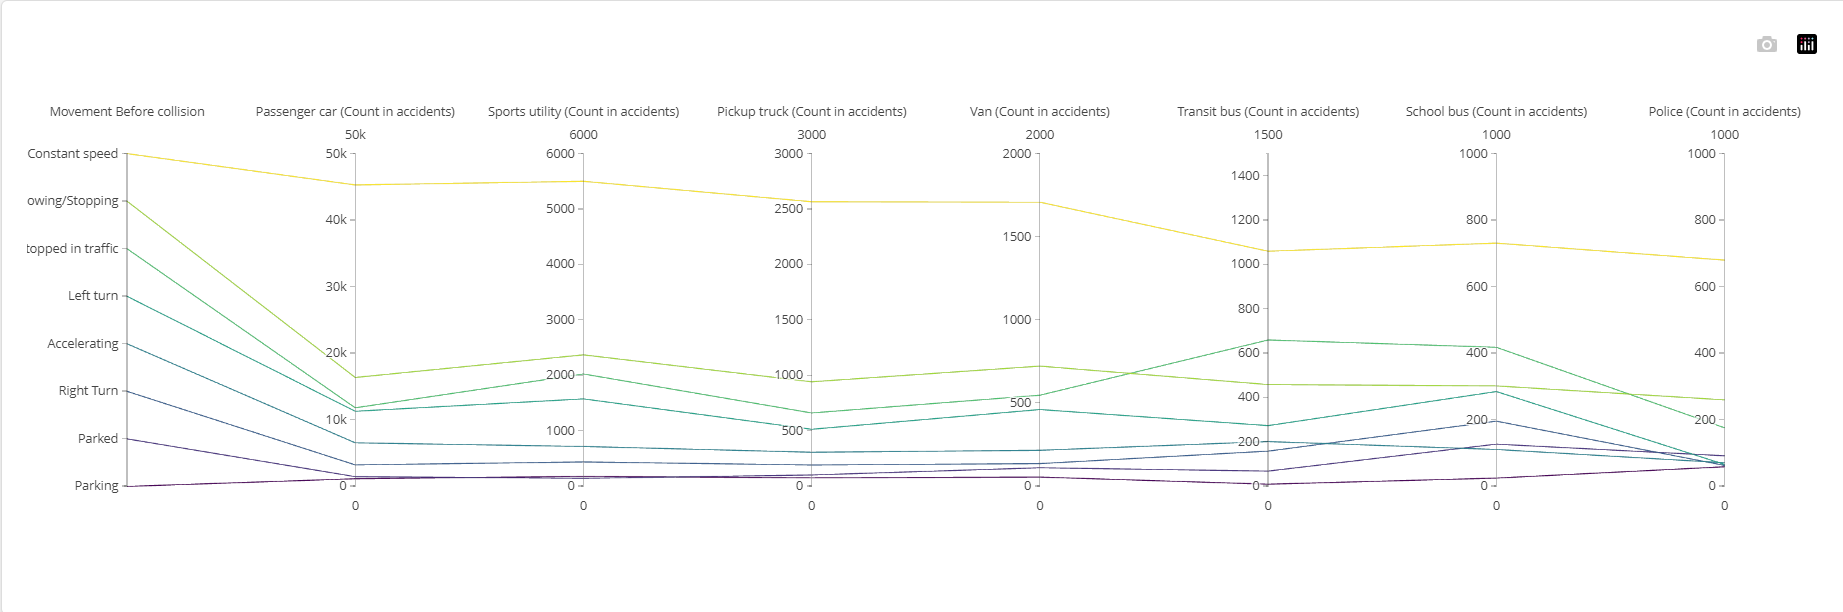
\includegraphics[width=1\linewidth]{pic1.png}
    \caption{Vehicle Type, Lighting Affecting Vehicle Accidents}
    \label{fig:enter-label}
\end{figure*}

From the provided parallel coordinates graph, which compares the count of accidents across different light conditions and vehicle types, several trends can be inferred:

\textbf{Light Conditions Impact on Accident Frequency:}
\begin{itemize}
    \item Daytime sees the highest number of accidents for passenger cars, which is expected as there are typically more cars on the road during this time.
    \item The difference between daytime and dark (with lights on) is not as pronounced for sports utility vehicles, vans, and pickup trucks, suggesting that these types of vehicles may be involved in accidents more evenly throughout different light conditions.
    \item The least number of accidents occur at dawn and dusk across all vehicle types, which could be due to fewer vehicles on the road during these times.
\end{itemize}

\textbf{Vehicle Type and Accident Correlation:}

\begin{itemize}
    \item Passenger cars are consistently involved in more accidents than any other vehicle type across all light conditions, likely due to their prevalence on the roads.
    \item Sports utility vehicles have a high count in accidents during the daytime but a significantly lower count during dark (lights on), indicating that they might be safer to drive or less commonly driven at night.
    \item Pickup trucks and vans show a similar pattern to each other, with counts decreasing less dramatically from daytime to dark (lights on) compared to passenger cars and sports utility vehicles.
\end{itemize}

\textbf{Public Transport Vehicles:}
\begin{itemize}
    \item Transit buses and school buses have a lower incidence of accidents across all light conditions when compared to personal vehicles.
    \item This could be due to the professional training of bus drivers, the larger size of the vehicle which may deter risky behavior from other drivers, or the fact that they are on the road for fewer hours per day compared to personal vehicles.
    \item Interestingly, the accident count for school buses is much higher during daytime than at night, probably due to most school timings being during the daytime.
\end{itemize}

\textbf{Emergency Vehicles:}
\begin{itemize}
    \item Police vehicles have a relatively lower count of accidents but seem to be involved in more accidents during the night (with lights on), which could correlate with high-speed pursuits or emergency responses during these times.
\end{itemize}

The graph illustrates the relationship between light conditions and accident counts while considering the type of vehicle involved. To make comprehensive inferences, it would be essential to consider external factors such as traffic volume, weather conditions, and geographic location. Additionally, the actual number of vehicles on the road for each category during the different light conditions would be needed to understand the accident rates properly. Without this contextual information, the inferences drawn are speculative and based solely on the visual data representation provided.\\

\textbf{B) Vehicle Type, Movement Affecting Vehicle Accidents}


\begin{figure*}
    \centering
    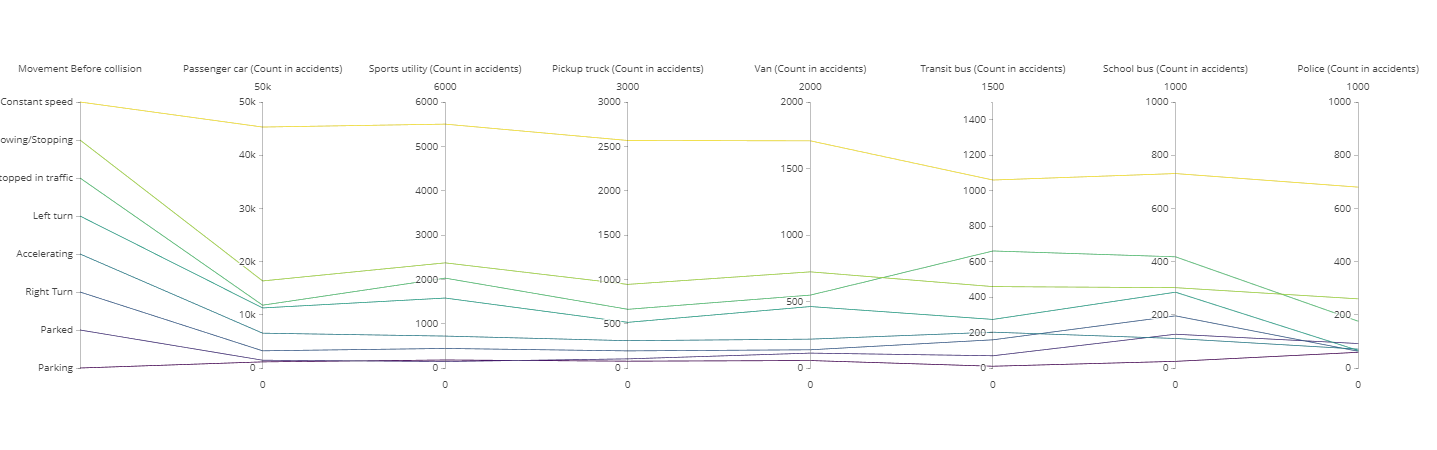
\includegraphics[width=1\linewidth]{newplot (2).png}
    \caption{Vehicle Type, Movement Affecting Vehicle Accidents}
    
\end{figure*}

\textbf{Constant Speed:}
\begin{itemize}
    \item Passenger cars have the highest number of accidents while moving at a constant speed, likely due to their prevalence on the roads.
    \item Sports utility vehicles, pickup trucks, and vans also have significant accidents at constant speed but less so than passenger cars, reflecting their smaller numbers on the roads.
\end{itemize}

\textbf{Slowing/Stopping:}
\begin{itemize}
    \item There is a decrease in the number of accidents for all vehicle types during slowing or stopping movements.
    \item Transit buses show a relatively high number of accidents while slowing or stopping, possibly due to their frequent stops and the associated risk of rear-end collisions.
\end{itemize}

\textbf{Stopped in Traffic:}
\begin{itemize}
    \item Passenger cars and sports utility vehicles show a noticeable number of accidents when stopped in traffic, highlighting their vulnerability to collisions in congested conditions.
\end{itemize}

\textbf{Left Turn:}
\begin{itemize}
    \item A significant number of accidents occur during left turns for all vehicle types, as this maneuver often involves crossing oncoming traffic, leading to potential side-impact collisions.
\end{itemize}

\textbf{Accelerating:}
\begin{itemize}
    \item Fewer accidents occur during acceleration for all vehicles, possibly due to the shorter duration of this movement and more attentive driving.
\end{itemize}

\textbf{Right Turn:}
\begin{itemize}
    \item Right turns seem to be safer, with fewer accidents reported for all vehicle types, likely because they generally involve fewer conflicts with other traffic in right-hand drive jurisdictions.
\end{itemize}

\textbf{Parked and Parking:}
\begin{itemize}
    \item Minimal accidents are reported for vehicles that are parked or parking, as expected due to these being static or low-speed maneuvers with a reduced chance of collision.
\end{itemize}

\textbf{Special Cases - Public and Emergency Vehicles:}
\begin{itemize}
    \item Transit and school buses display a distinct pattern with a lower overall number of accidents but higher incidences in certain maneuvers like slowing/stopping and right turns, reflecting their unique operational patterns.
    \item Police vehicles maintain a consistent but low count of accidents across all movements, possibly due to advanced driver training and the use of warning equipment.
\end{itemize}

It is crucial to consider that the raw count of accidents does not factor in the total number of vehicles or the distance traveled. Additionally, without information on the severity of accidents or external factors such as weather conditions, traffic signals, or road designs, these observations are based on the assumption that the data is representative of the overall population of vehicles and their movements prior to accidents.\\

\textbf{C) Vehicle Type, Weather Affecting Vehicle Accidents}

\begin{figure*}
    \centering
    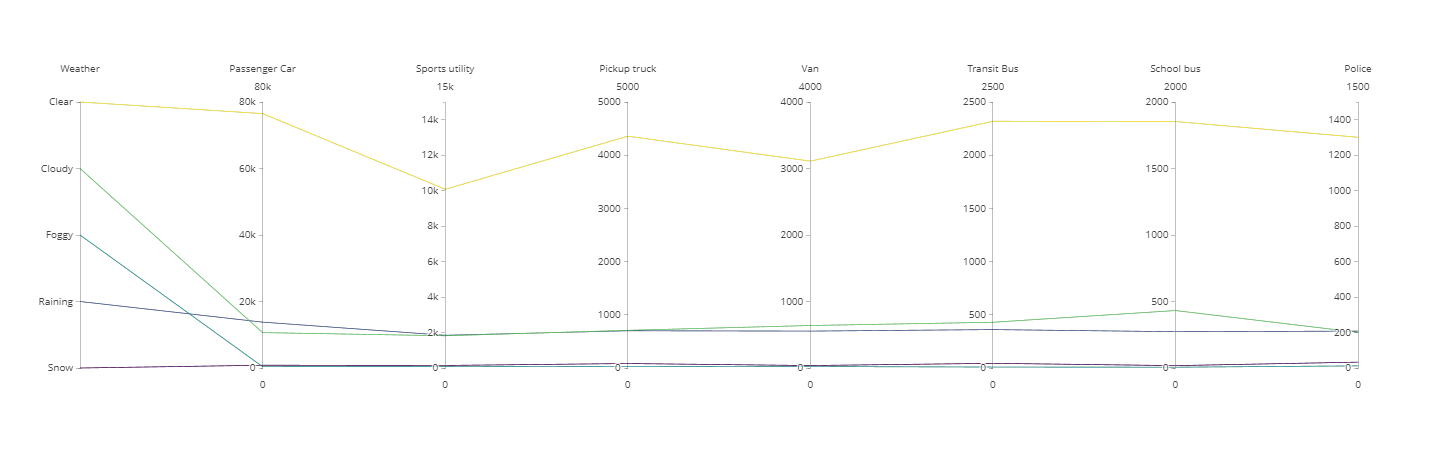
\includegraphics[width=1\linewidth]{newplot (3).png}
    \caption{Vehicle Type, Weather Affecting Vehicle Accidents}
    
\end{figure*}

\textbf{Weather Conditions:}
\begin{itemize}
    \item The highest number of accidents across all vehicle types occurs in clear weather, possibly due to increased traffic and less cautious driving.
    \item Cloudy conditions result in a lower but still significant number of accidents.
    \item In foggy and rainy conditions, accidents decrease further, suggesting increased driver caution or reduced traffic.
    \item Snowy conditions see the lowest accident counts, likely due to drastically reduced traffic and more cautious driving behavior.
\end{itemize}

\textbf{Vehicle Types:}
\begin{itemize}
    \item Passenger cars show the highest accident counts in all weather conditions, reflecting their higher numbers on the roads.
    \item Sports utility and pickup trucks experience fewer accidents as weather conditions worsen, perhaps due to better handling.
    \item Vans, transit buses, and school buses have lower overall accidents, potentially due to professional driving and limited operation hours.
    \item Police vehicles maintain a consistently low accident count, likely due to professional driving and vehicle readiness for diverse conditions.
\end{itemize}

\textbf{General Observations:}
\begin{itemize}
    \item There is a trend of decreasing accidents with worsening weather from cloudy to snowy conditions for all vehicle types, which may be influenced by a reduction in traffic volume and heightened driving caution.
\end{itemize}

\textbf{Justification:}
\begin{itemize}
    \item The analysis assumes that the data accurately reflects the number of accidents without considering the total number of vehicles on the road, which could impact the interpretation of accident rates.
    \item Thus, while poor weather might be expected to increase accidents, actual counts may be lower due to fewer drivers and more cautious behavior.
\end{itemize}

\item \textbf{ Tree Maps}
\begin{enumerate}
    \item \textbf{Vehicle Body Type, Injury Severity, Vehicle Make, Vehicle Damage Extent: }

    From the tree map provided in the figures [4, 5, 6, 7], which compares the accident frequency of different vehicle types and further delves into the vehicle maker, damage extent of the vehicle, and injury severity of the passenger, we can draw the following inferences:

    \textbf{Accident frequency of Vehicle Types: }
    \begin{itemize}
        \item Passenger vehicles are the most likely to get into accidents. They account for more than 70 percent of the accidents that happen. 
        
        \item This is expected because, in general, most of the cars on the road turn out to be passenger vehicles making them more likely to have accidents. The sheer number of passenger cars is a strong contributing factor to the observation.

        \item The next in line are SUVs, pickup trucks, vans,  and motorcycles, which are all, the most popularly used vehicles for common people.
    \end{itemize}
    
    \textbf{Passenger safety levels of different vehicle types:}
    
    \begin{itemize}
    \item Clicking on any of the tiles corresponding to vehicle body type in the tree map will update the tree map to display the distribution of accidents against injury severity of passengers. Thus, we can compare how safe different vehicle types are relative to each other using real-world crash data.

    \item We find that about 80 percent of passenger vehicle accidents had no injury involved, and the numbers for SUV vehicles also remain just about the same. This is a bit contradictory to the general dogma that SUVs are more safer on road than normal passenger vehicles. 

    \item Whereas, motorcycle accidents involve more injuries. About 77 percent of the total motorcyle accidents reported had passengers getting injured, with 20 percent of them getting seriously injured or fatally injured. This is quite understandable as 2-wheelers are less safer than other 4 or more wheeler vehicles, with no seat belts or airbags. 
    \end{itemize}

    \textbf{Popularity \& Safety of vehicles of various Vehicle Makers:}
    \begin{itemize}
    \item If we go a level deeper by clicking on one of the tiles, we can see a tree map that depicts the distribution of vehicles across different car-makers.

    \item This treemap is actually nested inside the corresponding rectangle in the injury severity treemap, which is nested inside its corresponding rectangle in the vehicle body tree map. This also theoretically helps us to infer the safety levels of various car makers along with their popularity. But we will only be inferring the popularity because the number of accidents is strongly influenced by the popularity of the vehicle under every scenario. 
    
    \item The most popular car maker (for passenger cars and SUVs) happens to be Toyota, followed by Honda, Ford, Nissan, and other popular car makers like Chevrolet and BMW. When it comes to pick-up trucks Ford takes first place in the ranking, with Toyota in the second. For motorcycles, Honda is the most popular followed by BMW.
    
    \end{itemize}
    
    \begin{figure}
        \centering
        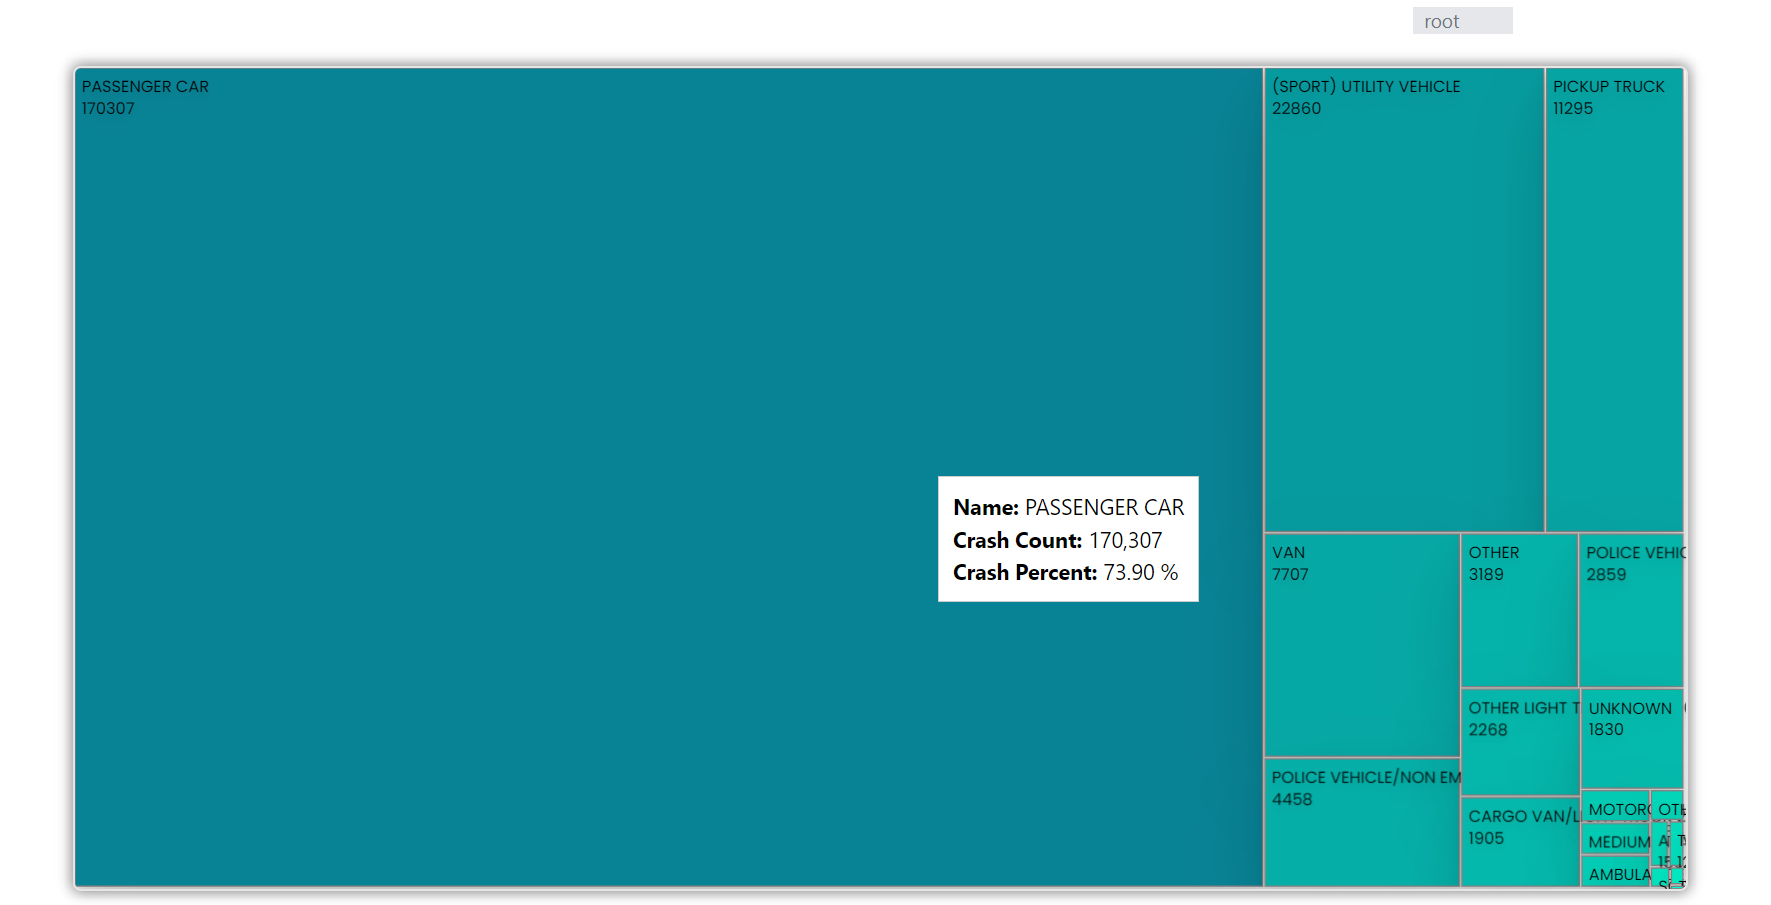
\includegraphics[width=1\linewidth]{tree-map1_level1.png}
        \caption{Tree map 1: First Level }
        \label{fig:enter-label}
    \end{figure}
    \begin{figure}
        \centering
        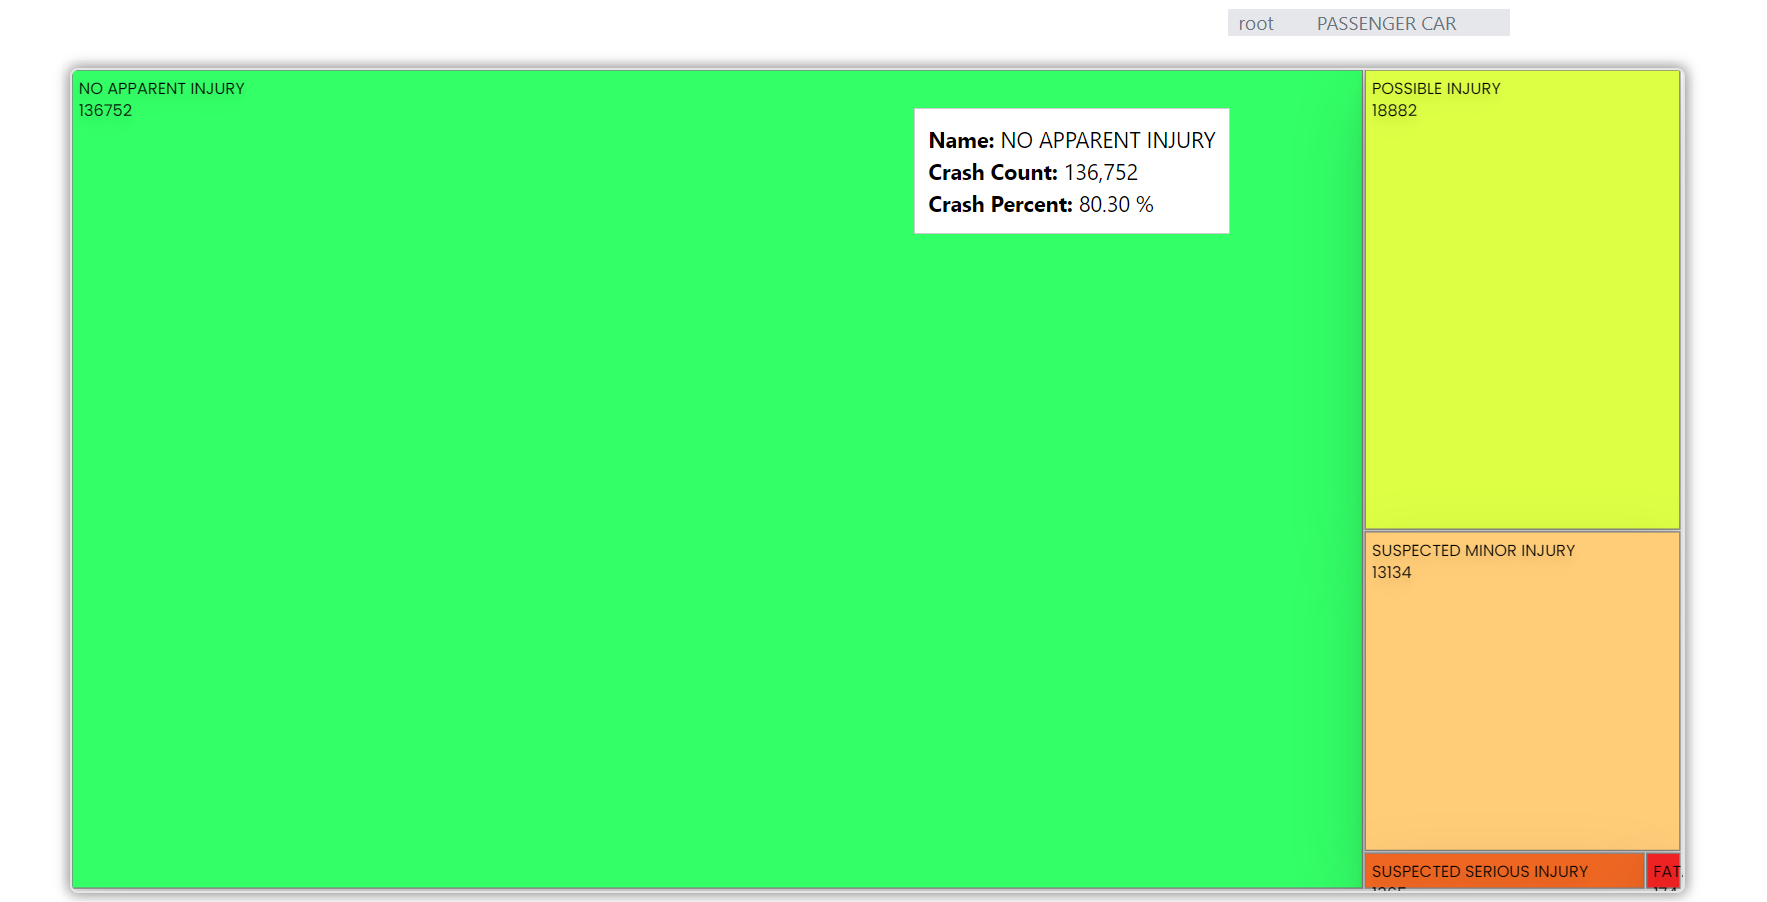
\includegraphics[width=1\linewidth]{tree-map1_level2.png}
        \caption{Tree map 1: Second Level }
        \label{fig:enter-label}
    \end{figure}
    \begin{figure}
        \centering
        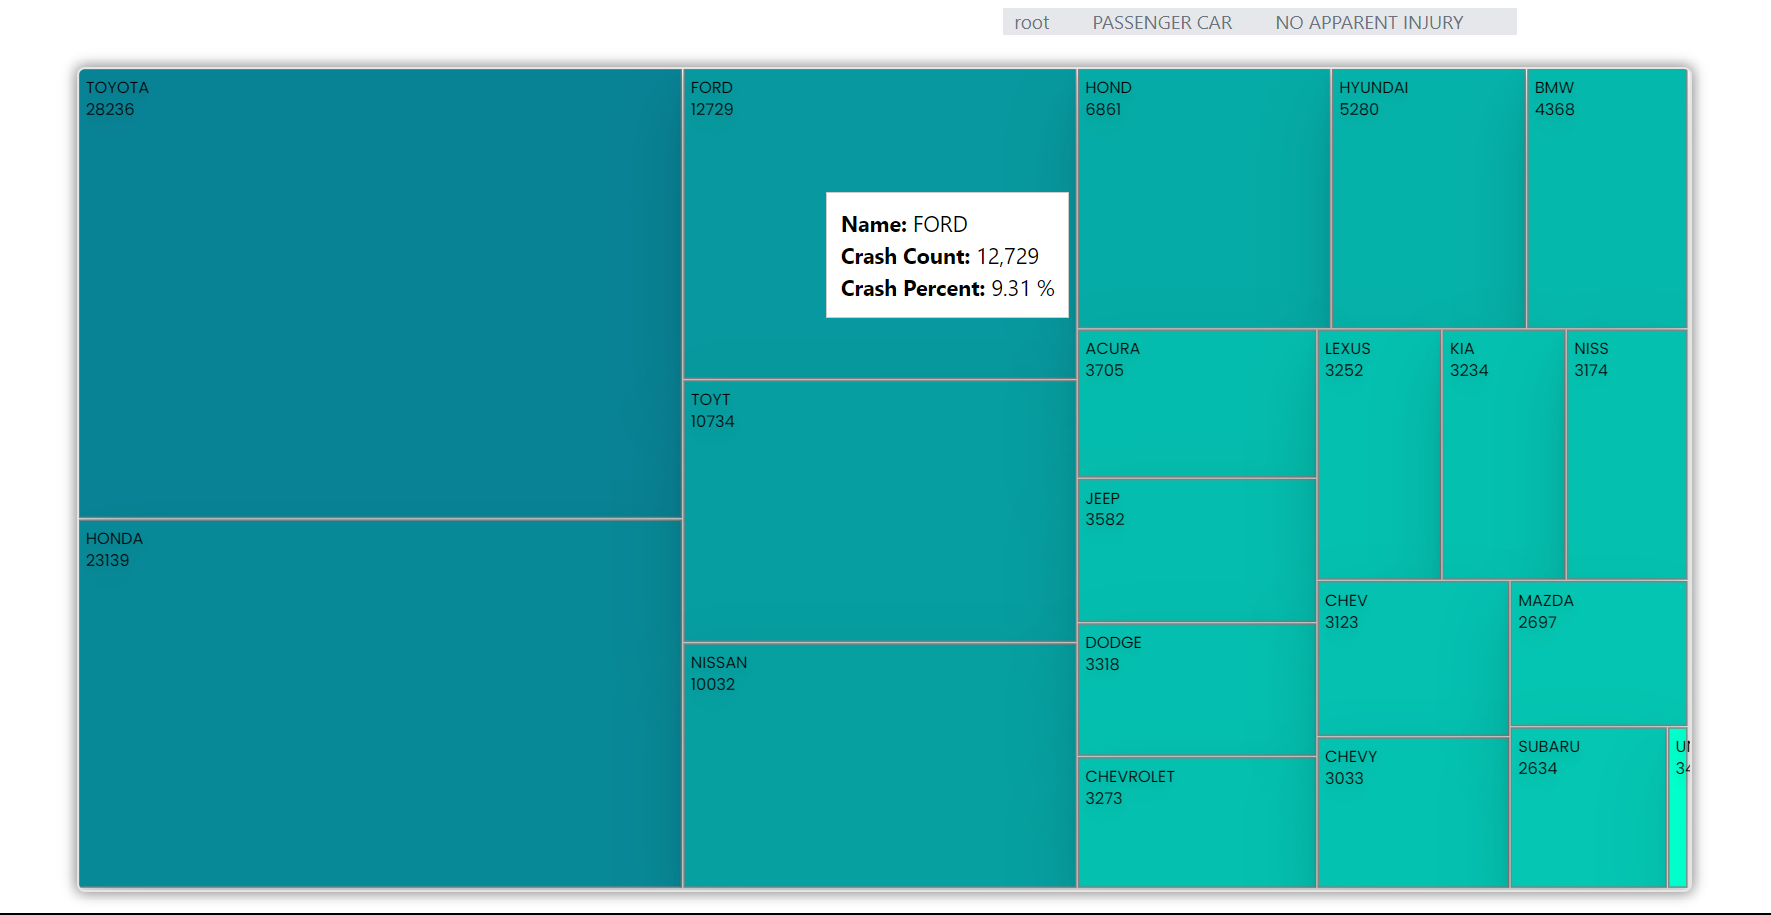
\includegraphics[width=1\linewidth]{tree-map1_level3.png}
        \caption{Tree map 1: Third Level }
        \label{fig:enter-label}
    \end{figure}
    \begin{figure}
        \centering
        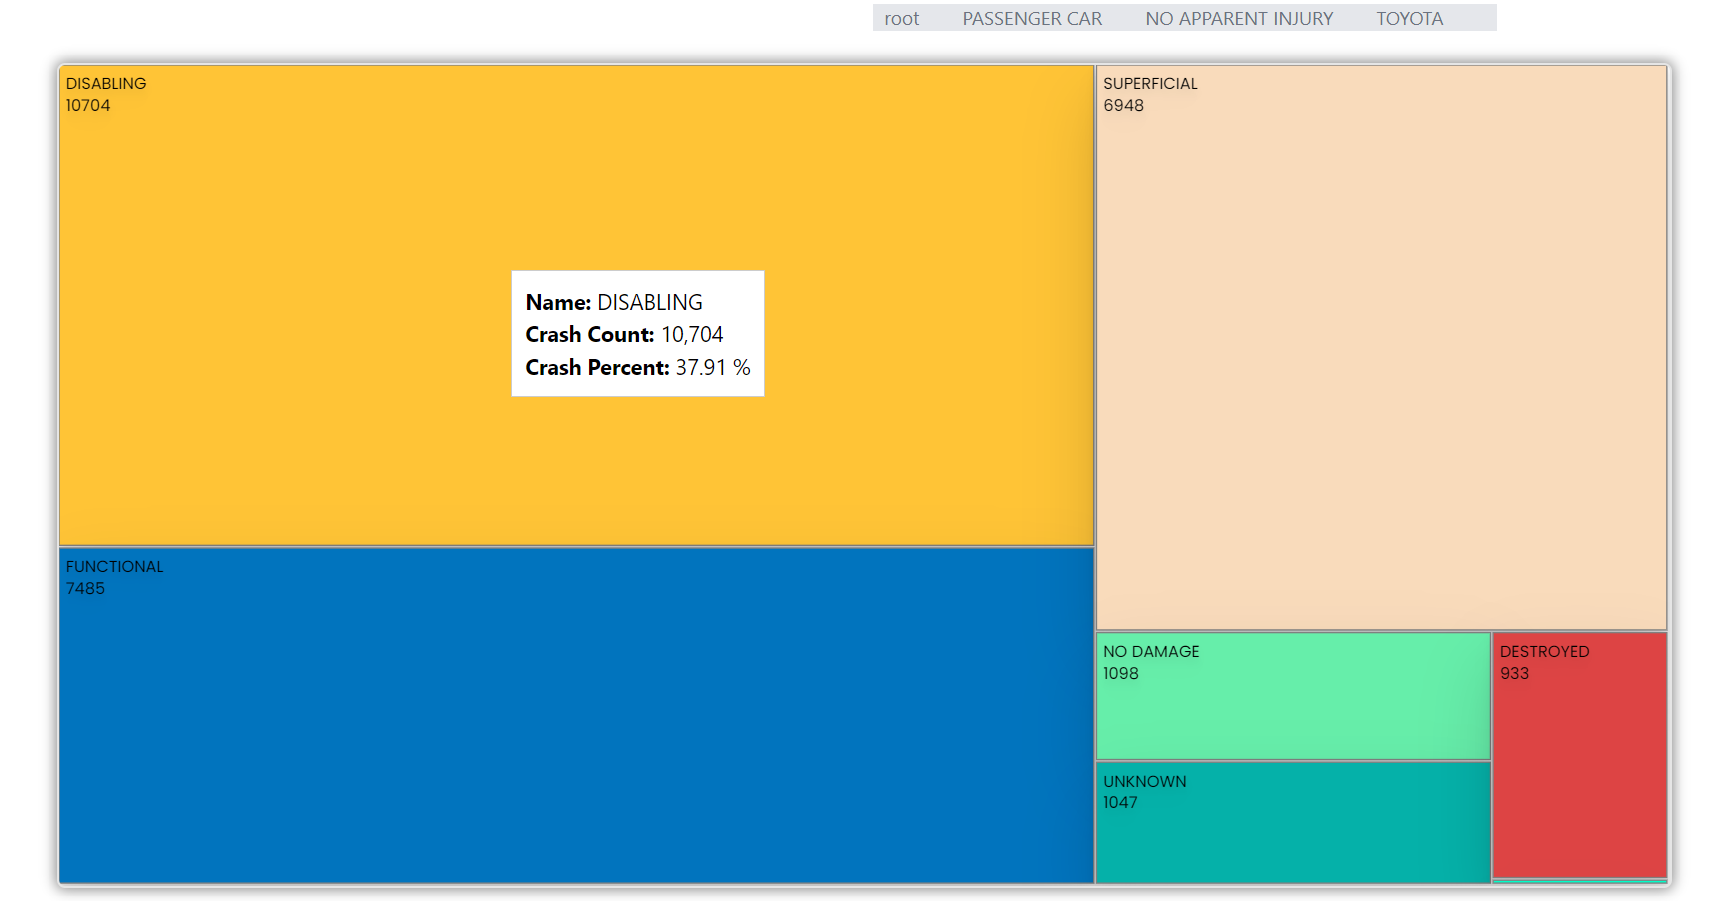
\includegraphics[width=1\linewidth]{tree-map1_level4.png}
        \caption{Tree map 1: Fourth Level }
        \label{fig:enter-label}
    \end{figure}
    
    \item \textbf{Vehicle Crash Year and Municipality: }
    From the tree map provided in Figures [8, 9], we can infer the following :
        
    \begin{itemize}
        \item The treemap tries to categorize data using the year and Municipality in which the crash was reported. From the tree map, we can infer which year has reported the highest crashes, and how the municipalities rank relative to each other in a given odd year.

        \item Like everything else, the number of accidents in a municipality is influenced by the number of vehicles on the road and the traffic. The traffic in a particular area is again influenced by its size and prominence. The ranking of municipalities (by number of accidents) remains the same across all the years (even and odd).

        \item The number of accidents does not seem to increase or decrease over time. Instead, it remains almost the same at an average range of 1200-1300 accidents per year. The year 2023 should be given lesser weightage as the data is not complete and the crash data for 2023 is only until August. This indicates that the positive increasing effect of growing traffic on vehicle crashes is being cancelled by the effect of improving road safety systems, traffic controls, and vehicle safety systems.
    \end{itemize}

    \begin{figure}
        \centering
        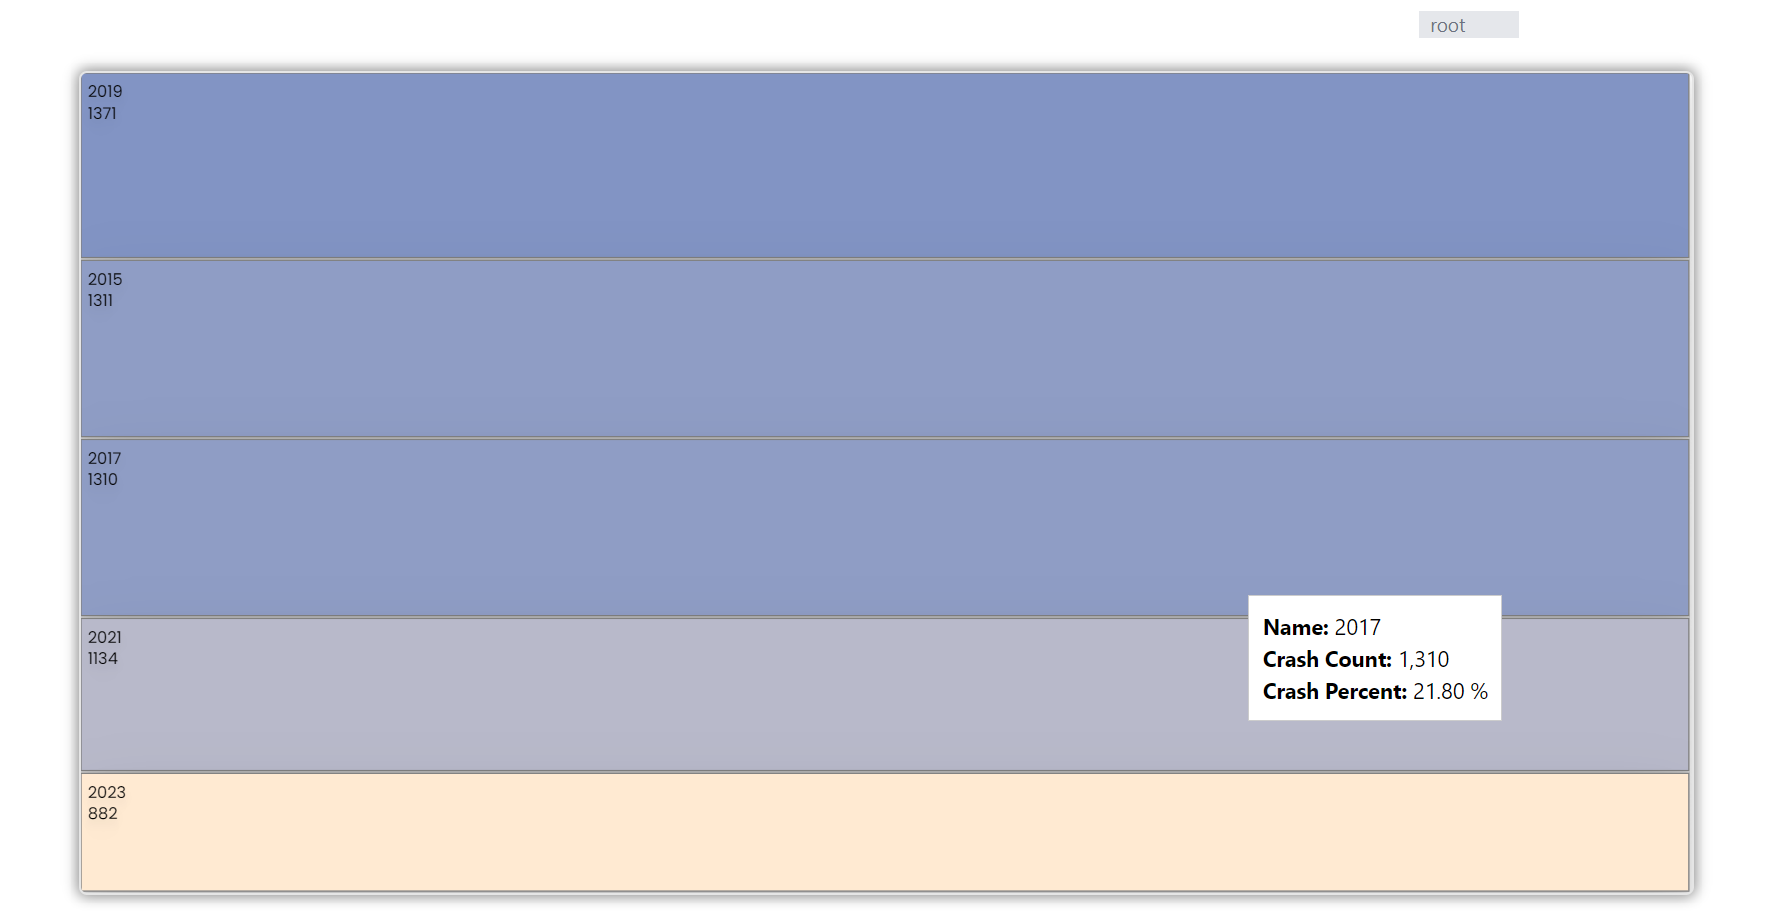
\includegraphics[width=1\linewidth]{tree-map2_level1.png}
        \caption{Tree map 2: First Level }
        \label{fig:enter-label}
    \end{figure}
    \begin{figure}
        \centering
        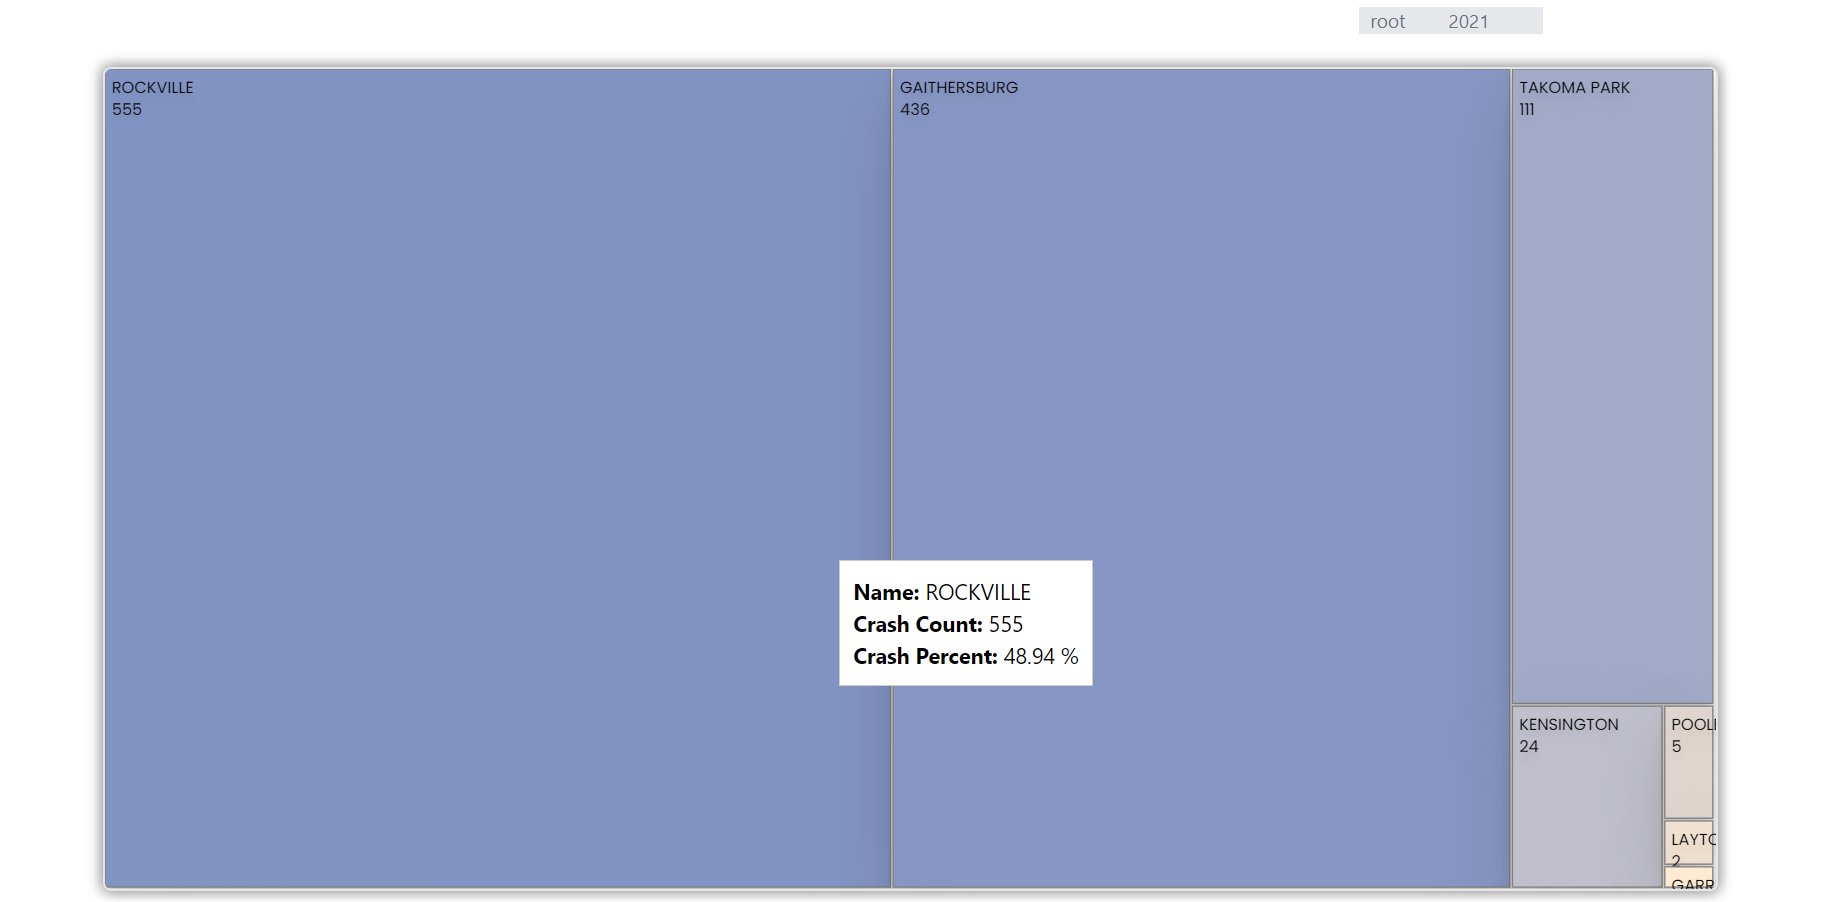
\includegraphics[width=1\linewidth]{tree-map2_level2.png}
        \caption{Tree map 2: Second Level }
        \label{fig:enter-label}
    \end{figure}
    
    
    \item \textbf{Driver License State and ACRS report type: }
    This treemap is shown in Figures [10, 11]. This categorizes data based on the crash type reported and shows the categorical values using sizes of rectangles in the treemap. From the figure, we can infer: 

    \begin{itemize}
        \item The ratio of property damage crashes vs injury damage crashes. The first category is a collection of crashes that involve only property damage and no injuries to passengers involved in the accident. The second one includes injury damage, which means there may be property damage but there was definitely at least 1 passenger who was injured as a result of the crash. The Property damage is not as serious as injury damage (keeping in mind the importance of passenger safety over vehicle damage costs). The ratio of property to injury damage is 2:1, which is ok, and needs to be analysed carefully to mitigate loss due to damage in future accidents.

        \item In this tree map, we take a slightly different path to analyse the distribution of accidents across driver license states under each category. Here, by driver's license state, I refer to the state which issued the driving license to the driver. This could be the driver's home state. As expected drivers of Maryland (home state drivers) account for most of the accidents. This is again because of the fact that most of the drivers on the road are usually from their home state with relatively fewer drivers visiting from other states. The ranking of states can be inferred from the tree map.
        For the reference of readers and TAs evaluating the submission, I have inserted a link in the HTML file of the tree map, that takes you to a page that lists all the state codes and their respective state names in tabular format.
    \end{itemize}
\end{enumerate}


\begin{figure}
        \centering
        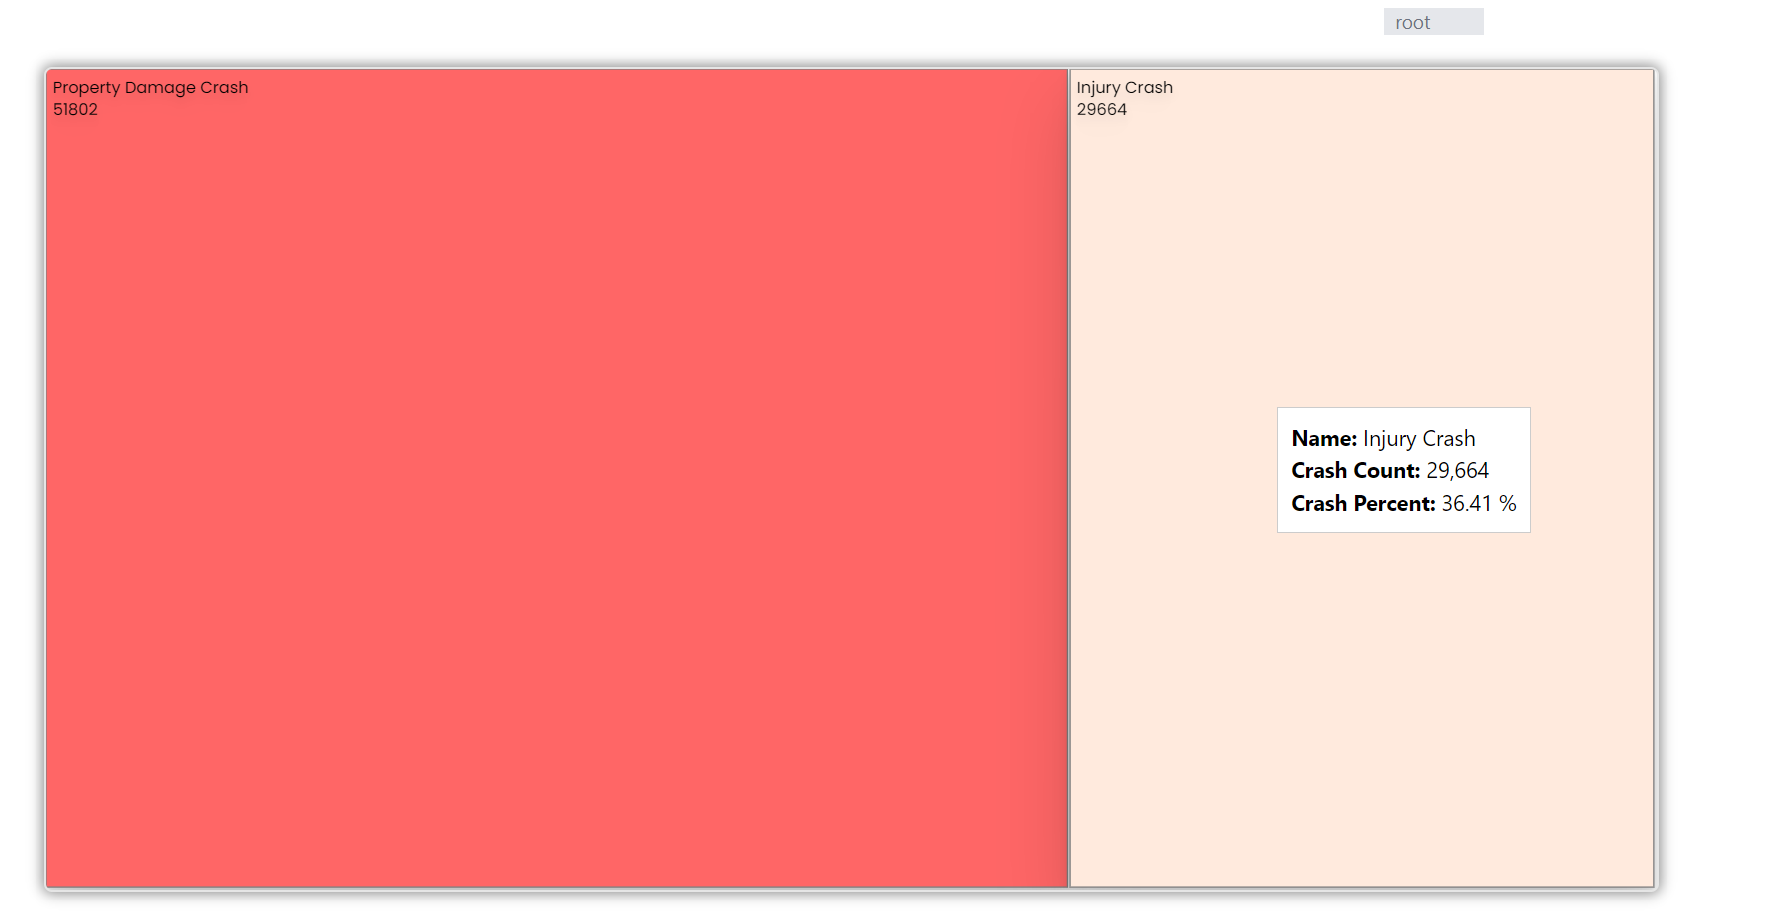
\includegraphics[width=1\linewidth]{tree-map3_level1.png}
        \caption{Tree map 3: First Level }
        \label{fig:enter-label}
    \end{figure}
    \begin{figure}
        \centering
        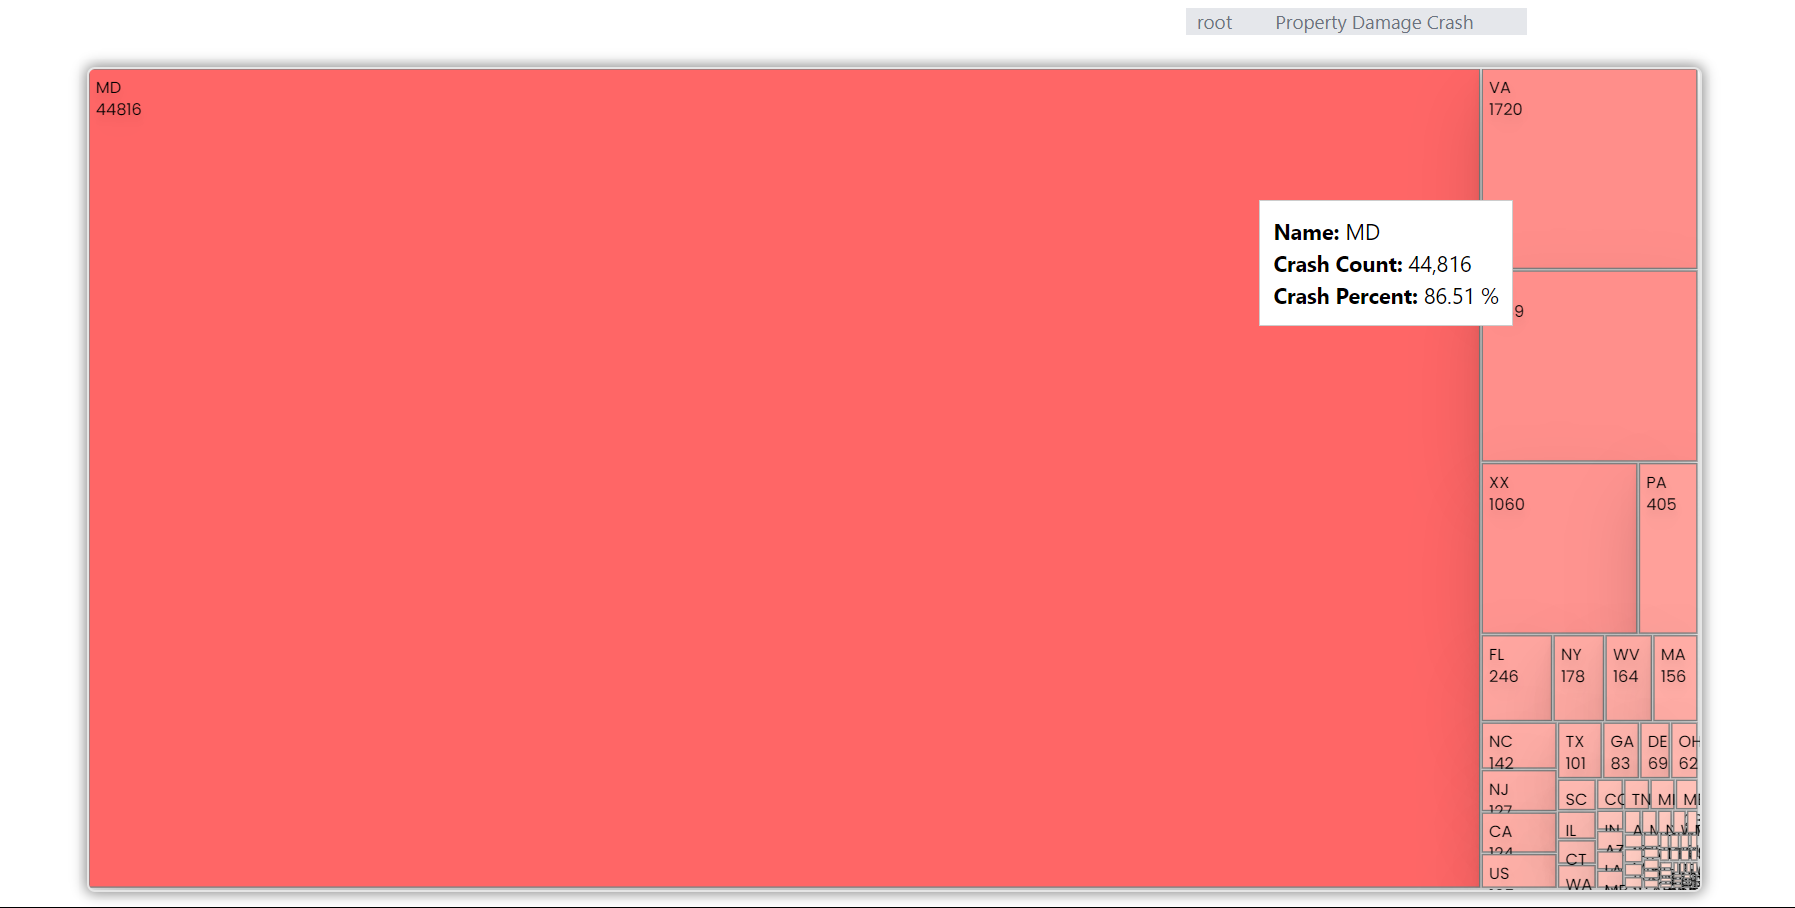
\includegraphics[width=1\linewidth]{tree-map3_level2.png}
        \caption{Tree map 3: Second Level }
        \label{fig:enter-label}
    \end{figure}
    






    

    
    
\item \textbf{Node link Diagram}
\begin{enumerate}
    \item
    \textbf{Node In-Degree Analysis:} The size and color intensity of nodes show their in-degree. A larger, more vividly colored node suggests a member of Congress who aligns with many others, indicating a central or influential figure in terms of voting patterns (Fig 4,5).

    \item
    \textbf{Edge Color Analysis:} The blue and red edges indicate positive and negative votes, respectively. A dense cluster of blue edges would suggest a group of members consistently voting together affirmatively, while a cluster of red edges would indicate a group frequently voting in opposition (Fig 4,5,6).
 
    \item
    \textbf{Network Clusters and Topology:} The overall structure of the network—how nodes are clustered together, which nodes are central, and which are peripheral—can reveal factions within Congress, key influencers, and possible outliers or members who vote independently of larger groups.

    \item 
    \textbf{Dynamic Interactions:} The final layout can give insights into the dynamic interactions between members. Two nodes are pulled close together despite their connecting edges being red (Can be noticed in Fig 5,6 near the centre a network of closely placed red edge nodes), this might suggest a complex relationship where members often vote in opposition but are linked through other factors, such as shared committees or mutual connections. Such as being in the same party.


    \item
    \textbf{Spatial Distribution:} The spatial distribution of nodes can indicate polarization or consensus. For instance, we can see graph shows two distinct clusters on opposite sides with few interconnecting edges (Multiple such can be seen for Fig 4), it could reflect a polarized voting pattern. Conversely, a more homogeneous network with many interconnecting blue and red edges might indicate a high level of cross-party collaboration (Outer figure 5 shows homogeneity in minor political players ). We can see large, central nodes are connected primarily by blue edges, it suggests a cohesive voting block (Larger nodes in Fig 4,5 have such dense blue webs around them).

    \item 
    \textbf{Force atlas: }
    \begin{figure}
        \centering
        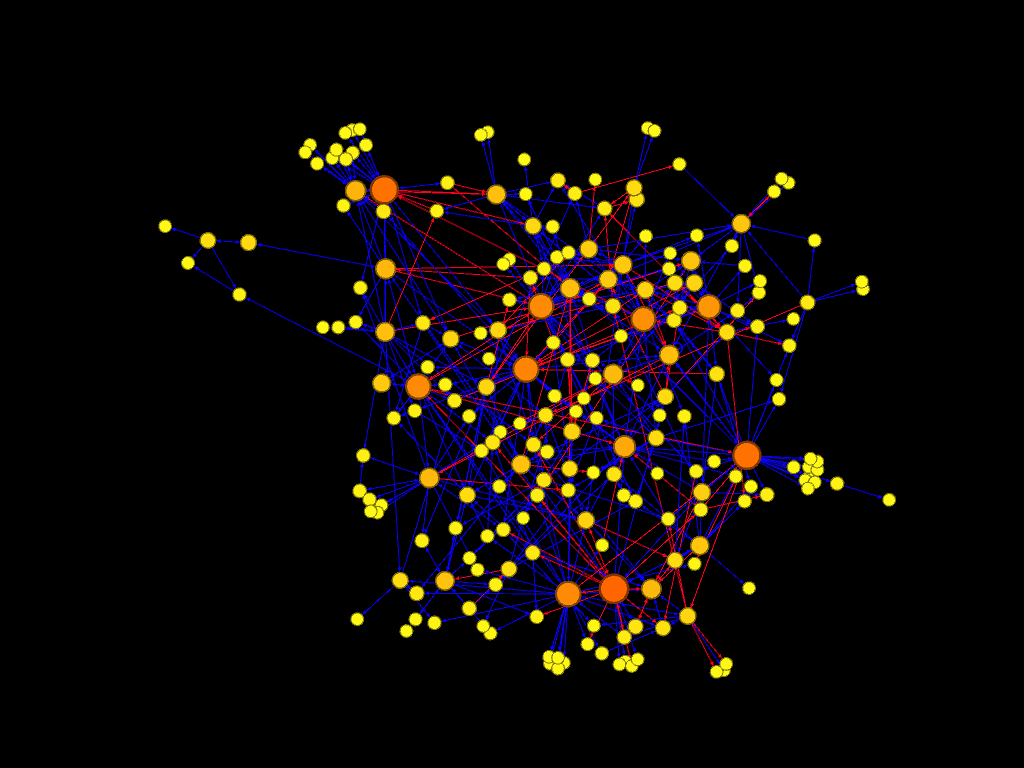
\includegraphics[width=1\linewidth]{ForceAtlas2_Dv_2.png}
        \caption{Force Atlas node link (Congress votes)}
        \label{fig:enter-label}
    \end{figure}
    The Force Atlas algorithm is a force-directed layout that treats edges like springs and nodes like charged particles, with attractive and repulsive forces applied to form a readable layout. This algorithm is particularly useful for such data because it:
    \begin{itemize}
        \item Reveals Structures: By allowing nodes to move to a position where forces are balanced, it uncovers the underlying structure of the network, such as communities or clusters.
  
        \item Adapts to Data: The algorithm is dynamic, meaning it can adapt to the specificities of the data-set, such as the number of nodes and the complexity of connections.
  
        \item Visual Clarity: Force-directed algorithms, like Force Atlas, spread nodes evenly and minimize edge crossings, which enhances visual clarity and readability.

        \item Interactive Exploration: The algorithm is iterative and can be run in real-time, allowing for interactive exploration of the network. This can be particularly useful for large data-sets (such as the one given to us) where the structure and patterns are not immediately obvious.
    \end{itemize}

    \item 
    \begin{figure}
        \centering
        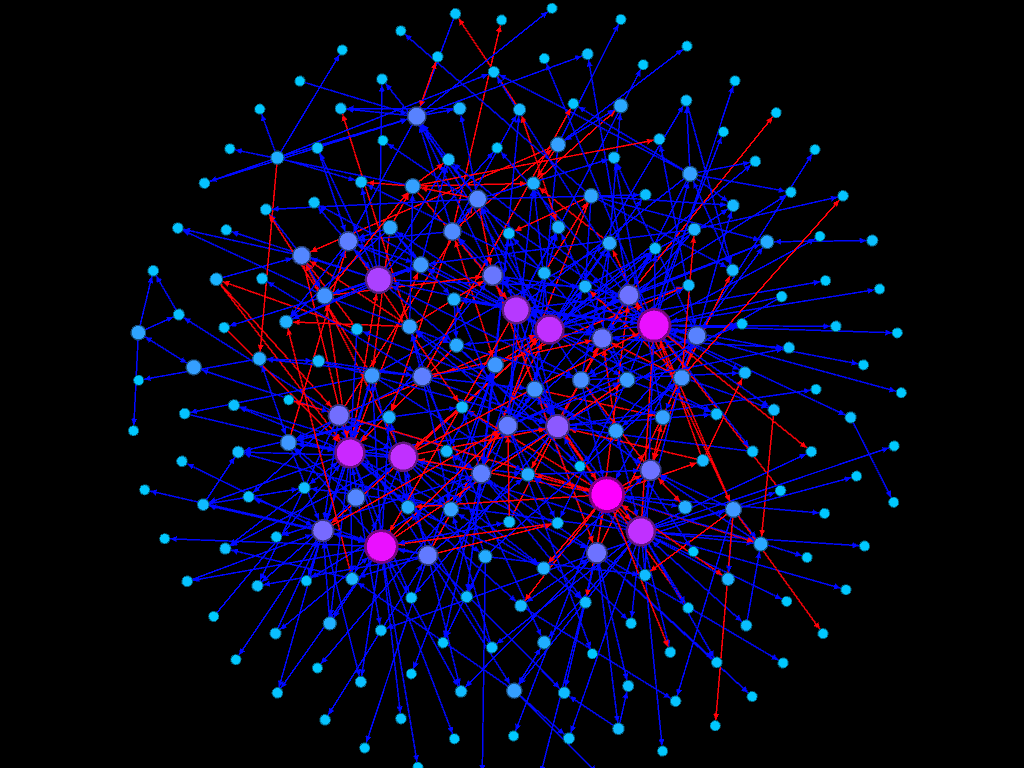
\includegraphics[width=1\linewidth]{Fruchter_NodeLink.png}
        \caption{Fructermann Reingold node link (Congress votes)}
        \label{fig:enter-label}
    \end{figure}
    \textbf{Fructermann Reingold: }
    \begin{itemize}
         \item This algorithm treats the nodes as if they are repelling each other while edges act like springs, creating an equilibrium state that helps to display the graph in a way that reflects the natural clustering within the data.
         \item It is particularly well-suited for visualizing data that may not have clear hierarchical structures (Not provided to us in simple edge node form) and is useful for emphasizing groupings and symmetries in the data.
         \item The algorithm aims to minimize edge crossings and make the layout as uniform as possible, which can make patterns of connection and disconnection within the network more apparent.
    \end{itemize}
    

    \item \textbf{Yifan hu}

    \begin{figure}
        \centering
        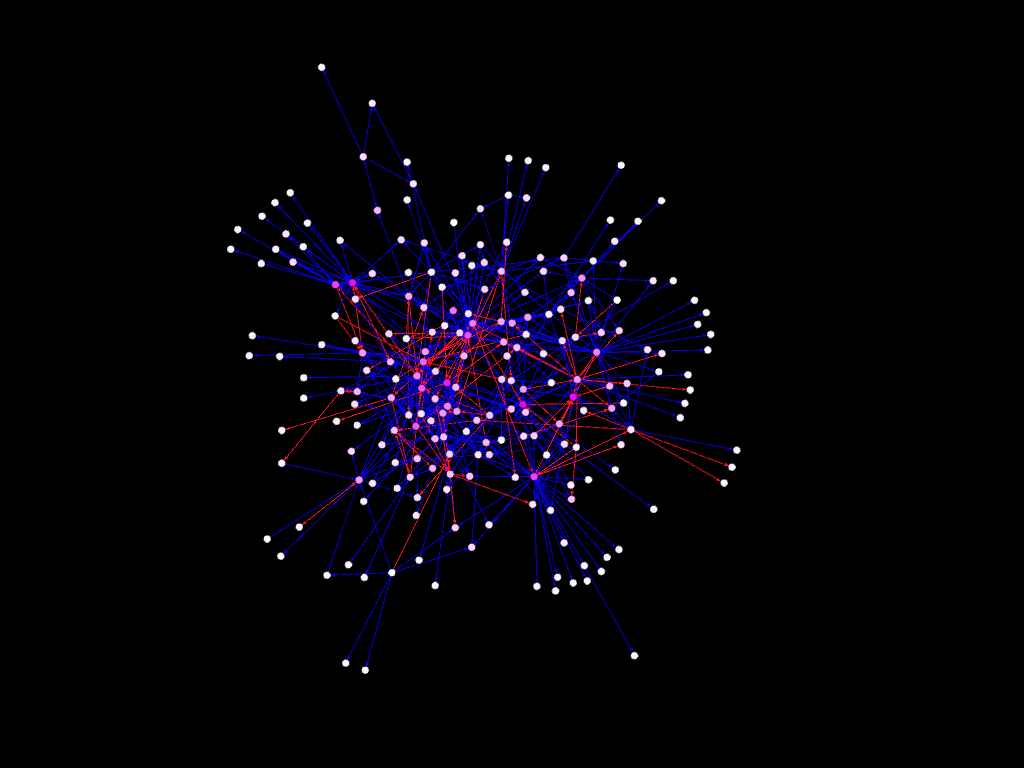
\includegraphics[width=1\linewidth]{Yifan_hu_Dv_2.png}
        \caption{Yifan hu node link (Congress votes)}
        \label{fig:enter-label}
    \end{figure}
    \begin{itemize}
        \item 
        The Yifan Hu algorithm is designed to work efficiently with large graphs, which makes it appropriate for complex datasets like congressional votes.
        \item
        It combines local and global optimizations to achieve high-quality visualizations with minimal clutter and good separation between nodes, making it easier to identify underlying patterns.
        \item
        It reduces the complexity of the visualization without oversimplifying the data, which helps in making clear inferences about the data.
    \end{itemize}

    


\end{enumerate}
    
    
    
    
    
    
\item Third item
\end{enumerate}


\subsection{Scivis}

As mentioned at the beginning of the report, same datasets were used for both the scivis tasks making writing non-overlapping inferences a genuinely difficult task. We have done our best to stay original to our inferences and opinions about the plots.
\begin{enumerate}

\item \textbf{Countour Plot}
Throughout the sequence of plots, there is a clear transition from lighter to heavier precipitation worldwide. The pattern of change from blue to green to red contours could indicate the seasonal progression of weather systems, including the start, peak, and intensity of rainy seasons or monsoonal patterns in different parts of the world.Following is the analysis for the Indian subcontinent (year 2015):
    \begin{itemize}
     

    \item \textbf{April 15 :} 
    \begin{figure*}
        \centering
        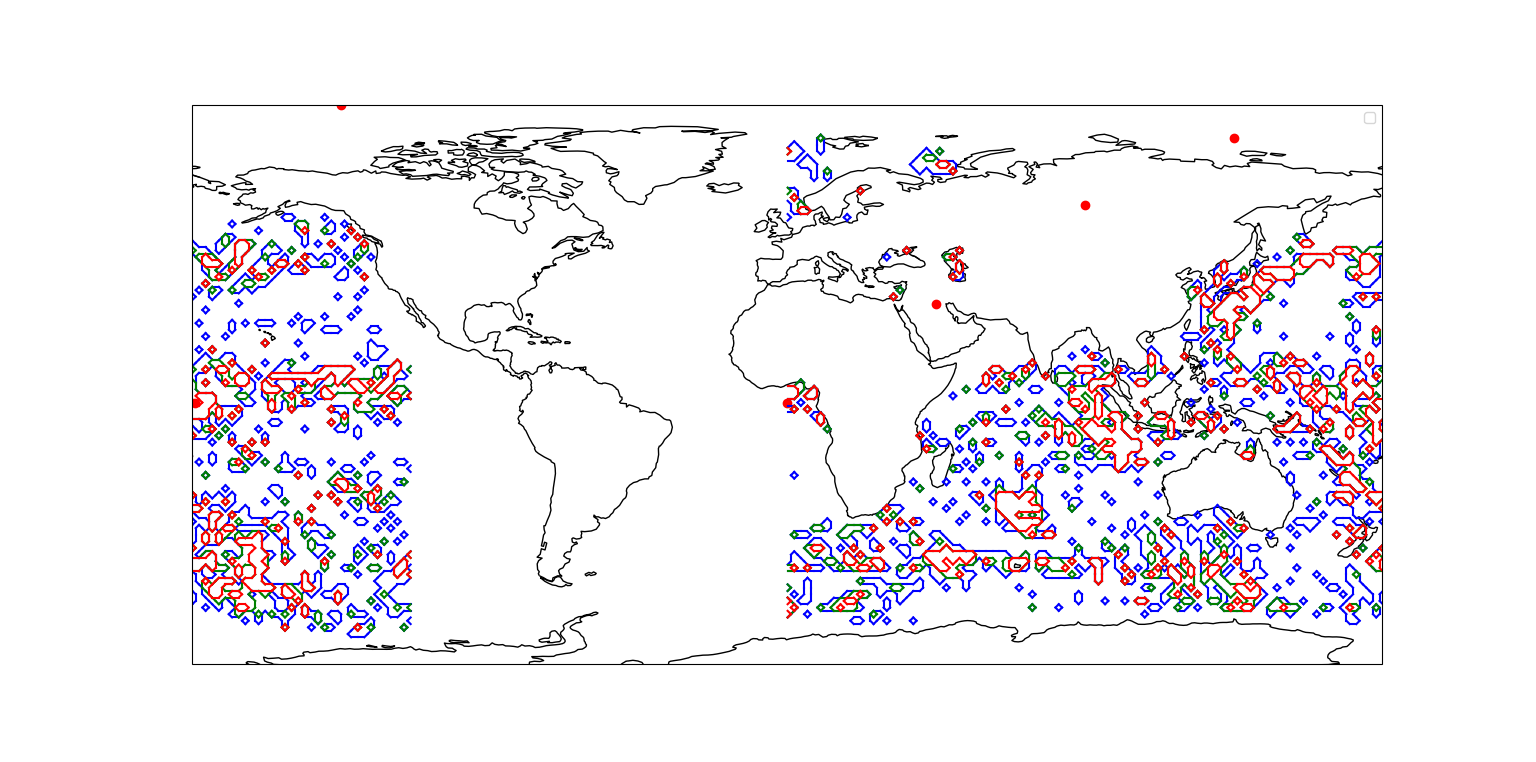
\includegraphics[width=1\linewidth]{Apr15.png}
        \caption{April 15}
        \label{fig:enter-label}
    \end{figure*}
    
    High rainfall region is indicated below India in the red contour.
    Hence we can conclude that normal rainfall i occurring and monsoon has not onset yet (Fig 7).

    \item \textbf{May 1 :} 
    \begin{figure*}
        \centering
        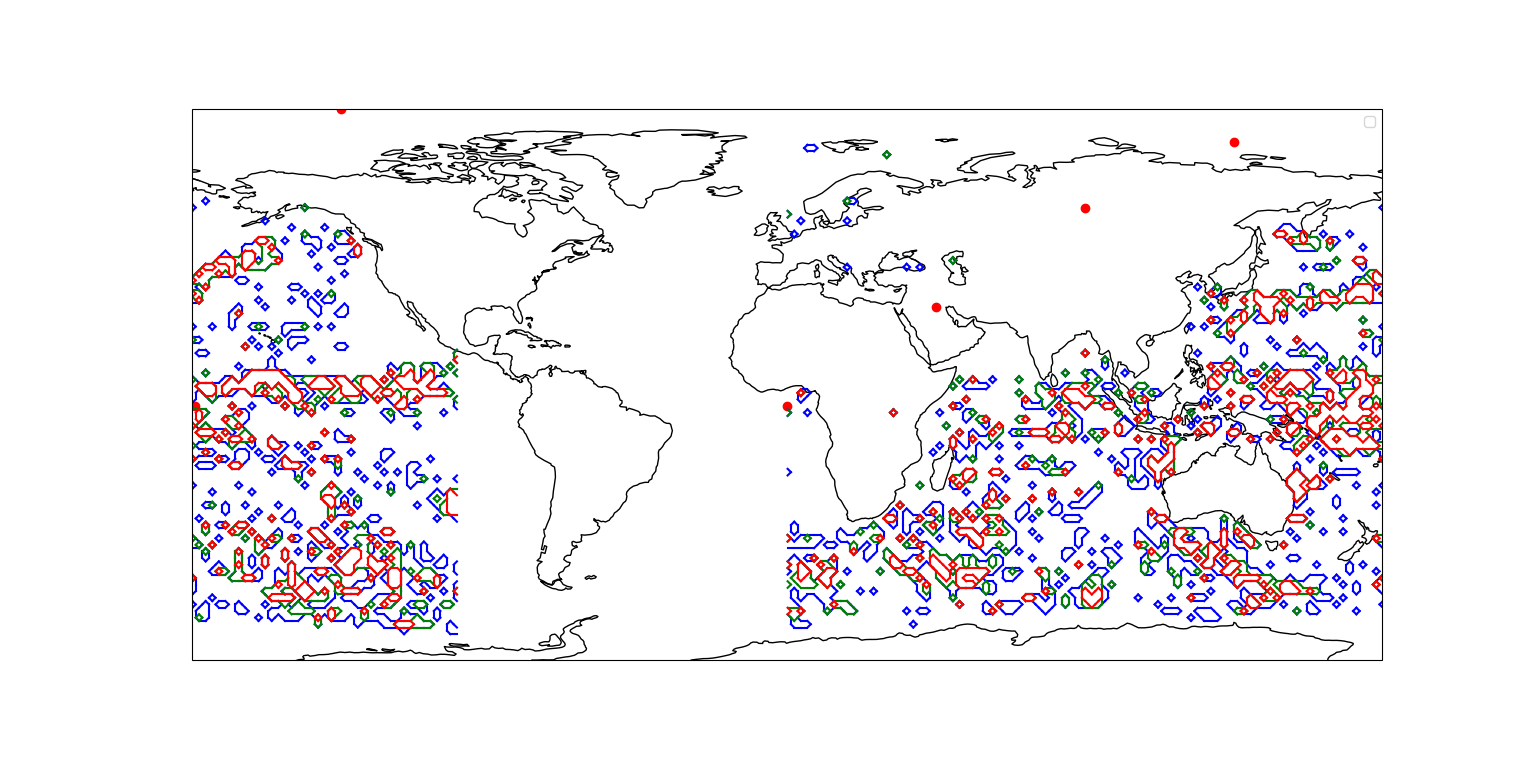
\includegraphics[width=1\linewidth]{May1.png}
        \caption{May 1}
        \label{fig:enter-label}
    \end{figure*}
    
    We can see the red rain belt approaching Sri-Lanka indicating that monsoon hasn't yet reached India but may affect southernmost parts of India (Fig 8).

    \item \textbf{May 11 :} 

     \begin{figure*}
         \centering
         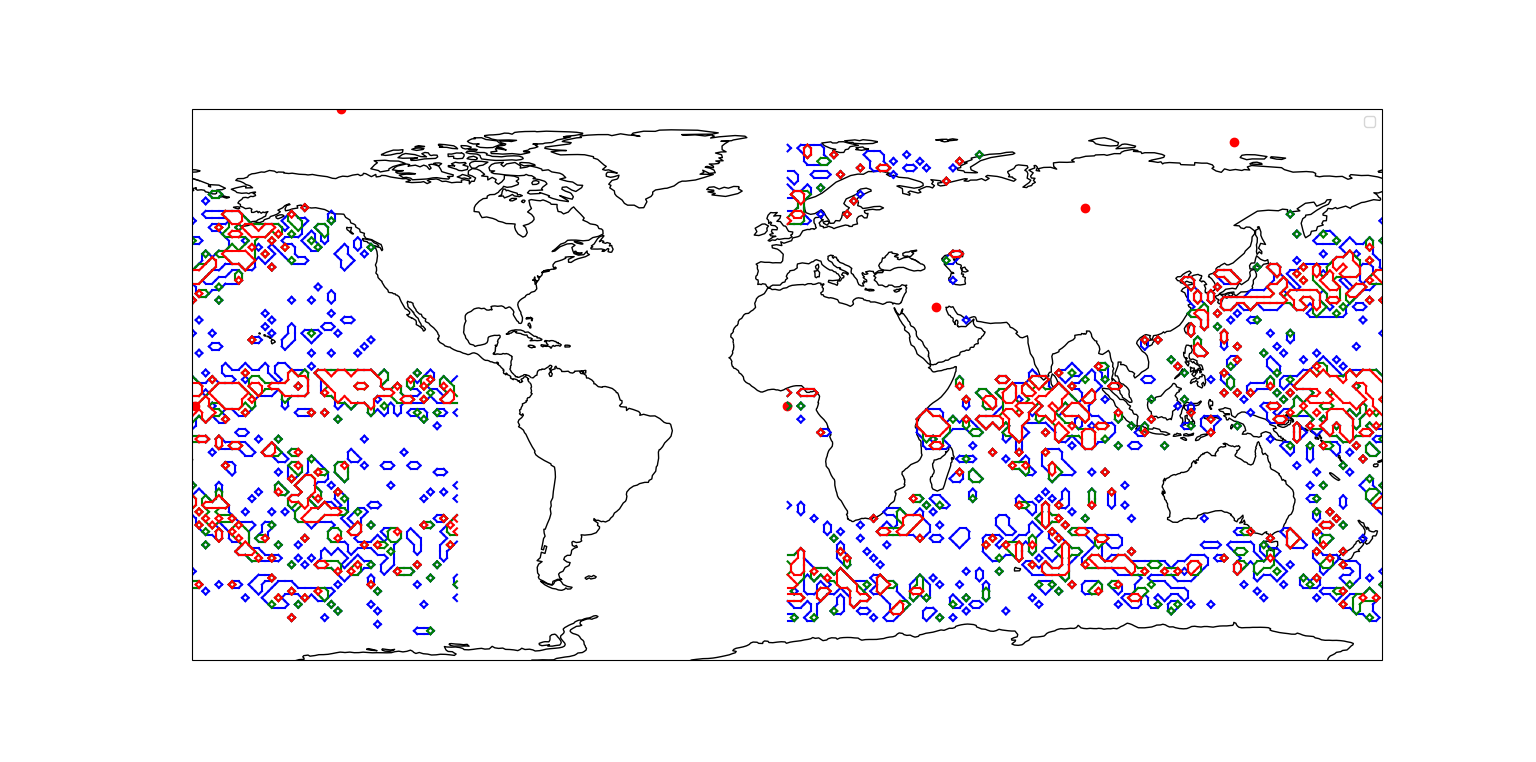
\includegraphics[width=1\linewidth]{May11.png}
         \caption{May 11}
         \label{fig:enter-label}
     \end{figure*}
    
    There is a great increase in the surface rain near South of india, indicating rising rainfall (Fig 9).

    \item \textbf{June 1 :} 
    
    \begin{figure*}
        \centering
        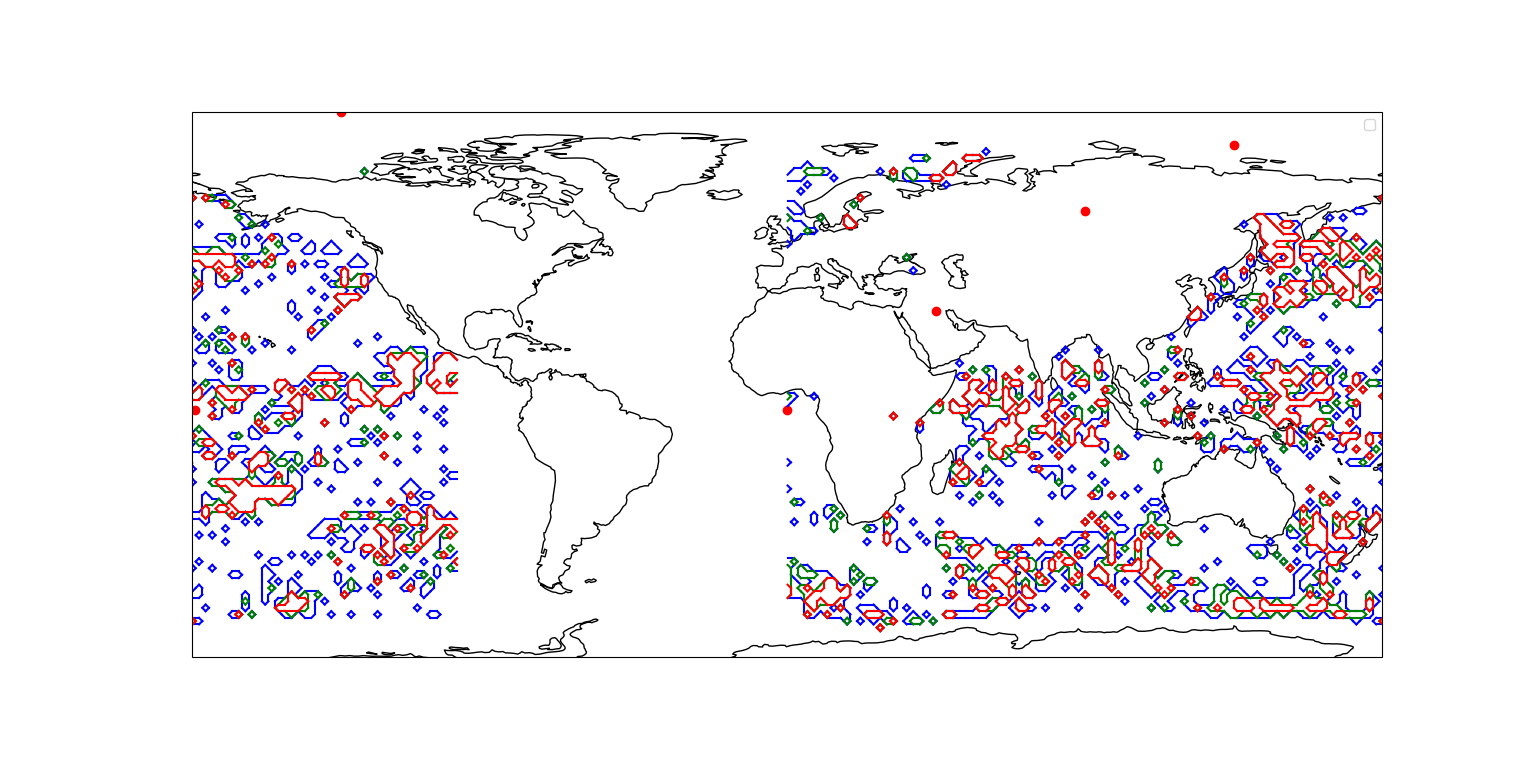
\includegraphics[width=1\linewidth]{Jun1.png}
        \caption{June 1}
        \label{fig:enter-label}
    \end{figure*}
    
    We can see that the red rain belt is now reached above near the more northern states of India, indicating the onset of monsoon in the north (Fig 10 ).

    \item \textbf{June 11 :} 
    
    \begin{figure*}
        \centering
        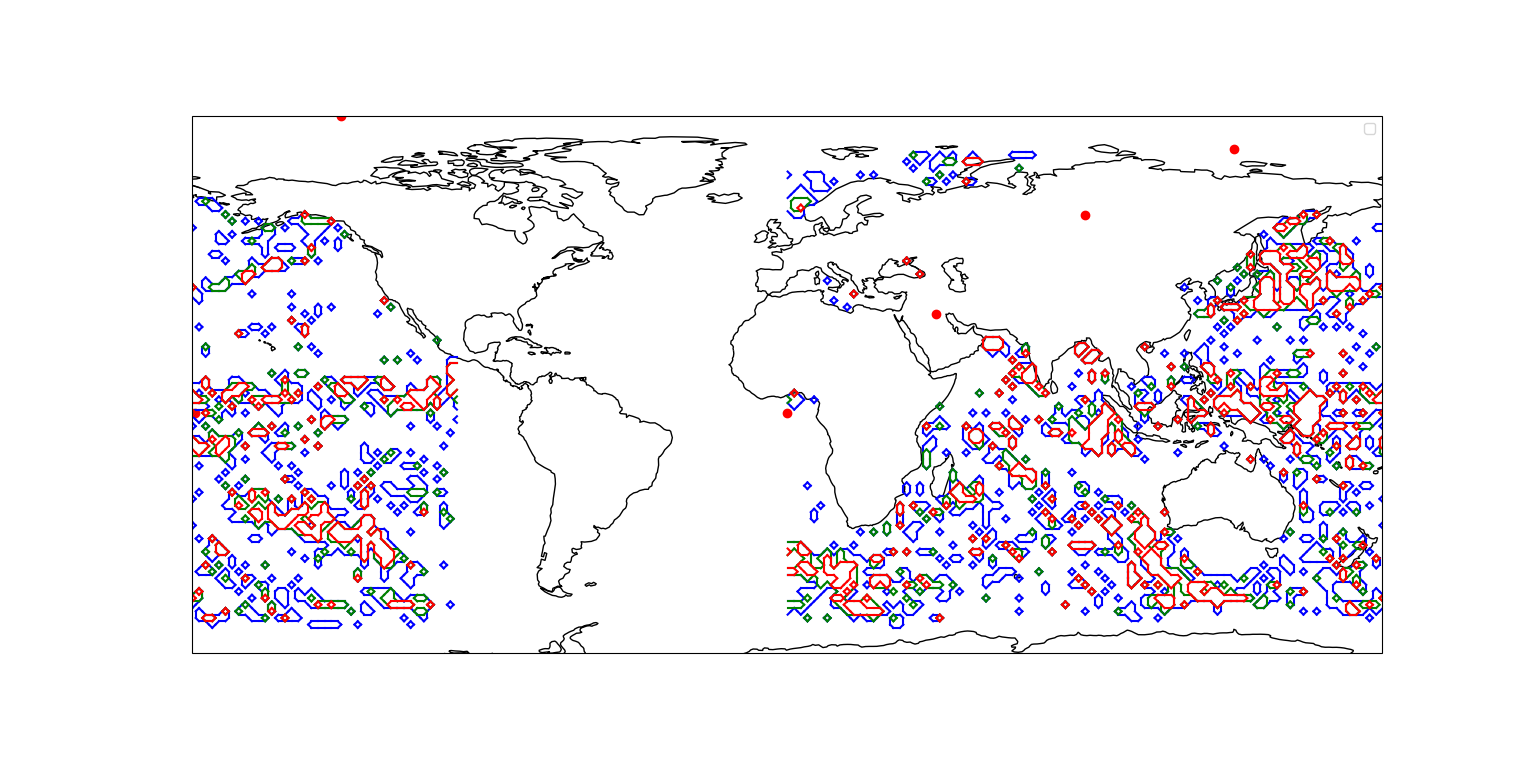
\includegraphics[width=1\linewidth]{Jun11.png}
        \caption{June 11}
        \label{fig:enter-label}
    \end{figure*}
    
    Now we can see red belts all around the Indian cost indicating heavy rain (Fig 11).

    \item \textbf{June 29 :} 
    
    \begin{figure*}
        \centering
        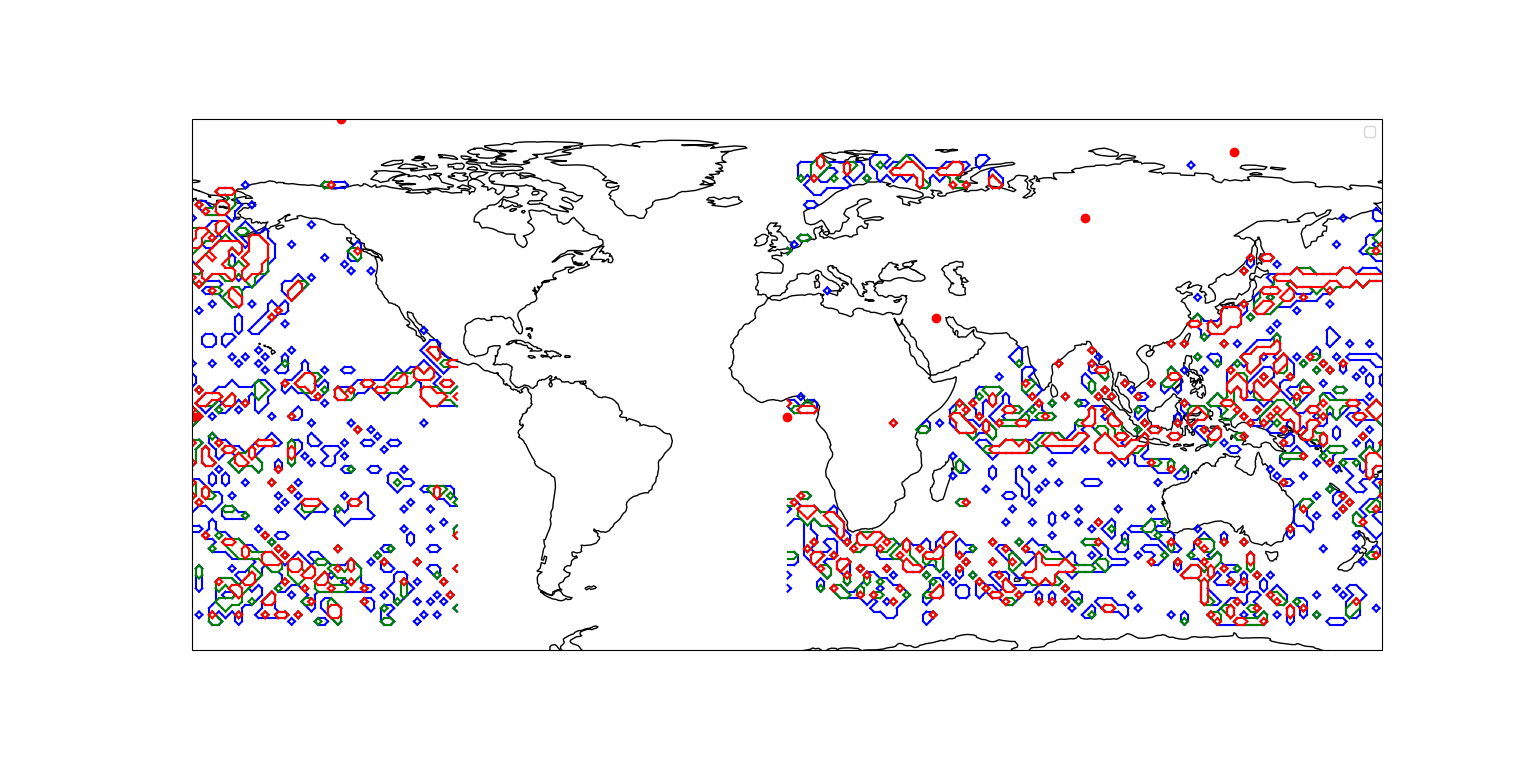
\includegraphics[width=1\linewidth]{Jun29.png}
        \caption{June 29}
        \label{fig:enter-label}
    \end{figure*}
    
    We can now see less red belts on the coast indicating that monsoon has finally reached the mainland and is crossing over Indian land (while reducing over the direct ocean comparatively) (Fig 12).\\

    \end{itemize}
 


    
\item \textbf{Color Map} 


\begin{enumerate}
\item \textbf{April 15:} The monsoon has not started yet, as it typically begins in June. Hence, the map shows minimal rain activity over the Indian subcontinent. The colour intensity over the Indian Ocean indicates pre-monsoon showers or climatic conditions leading up to the monsoon. (Fig. 21)

\item \textbf{May 1 and May 11:} The color maps for these 2 dates show some increase in activity, as the pre-monsoon season brings rainfall. If we look carefully at the color maps, we see some slight changes in colour over the Indian Ocean and the adjoining ocean area on May 11, indicating pre-monsoon rainfall. (Fig. 22, 23)

\item \textbf{May 21:} By this time, the effects of monsoon usually set in. Ideally, in the color map, the southwest of India (particularly over the Arabian Sea) should show increased rain activity. However, since the data is only a single sample and their could be abnormal days and hence this might not be very much visible in the color map. (Fig. 24)

\item \textbf{June 1:} This is around when the monsoon typically starts. We see a corresponding significant change in color over the southwestern coast of India. The rain appears to move inland, indicating the monsoon's arrival. (Fig. 25)

\item \textbf{June 11 and June 21:} By this time, the monsoon is well established over the southwestern and eastern parts of India. The color maps shows a clear shift in colors towards higher end of the scale, indicating high rain rates. Especially, on the Western Ghats and northeastern states, which typically recieves heavy rainfall. (Fig. 26, 27)
\end{enumerate}

Overall, to conclude the inference:
\begin{enumerate}
 \item A gradual intensification of rain rates from late May to June, moving from the southwest to the interior of India, indicates a normal progression of the Indian monsoon.
 \item The presence of high rain rates over the Bay of Bengal and the Arabian Sea can be seen in late June.

 \end{enumerate}
 
 This is our inference for contour and color map scivis tasks we have done.
\end{enumerate}





\section{Code}

\begin{enumerate}
\item 
\textbf{JavaScript Code for Parallel Coordinates Plots}

The JavaScript code defines three parallel coordinates plots using the Plotly library. Each plot (p1, p2, and p3) represents different aspects of accidents based on various dimensions. Here's an explanation of the code:

\begin{enumerate}
    \item \textbf{Plot 1 (p1): Light Conditions}
        \begin{itemize}
            \item Line Color: Varies based on the values [5, 4, 3, 2, 1] with a color scale from red to magenta.
            \item Dimensions: Light Conditions, Passenger Car, Sports Utility, Pickup Truck, Van, Transit Bus, School Bus, Police (Counts in accidents for each vehicle type).
        \end{itemize}
    \item \textbf{Plot 2 (p2): Movement Before Collision}
        \begin{itemize}
            \item Line Color: Varies based on the values [8, 7, 6, 5, 4, 3, 2, 1] with a color scale from red to blue.
            \item Dimensions: Movement Before Collision, Passenger Car, Sports Utility, Pickup Truck, Van, Transit Bus, School Bus, Police (Counts in accidents for each vehicle type).
        \end{itemize}
    \item \textbf{Plot 3 (p3): Weather Conditions}
        \begin{itemize}
            \item Line Color: Varies based on the values [5, 4, 3, 2, 1] with a color scale from red to blue.
            \item Dimensions: Weather Conditions, Passenger Car, Sports Utility, Pickup Truck, Van, Transit Bus, School Bus, Police (Counts in accidents for each vehicle type).
        \end{itemize}
\end{enumerate}


\textbf{Plotly.newPlot:}
\begin{itemize}
    \item Plotly.newPlot is used to create each parallel coordinates plot.
    \item The first argument is the ID of the HTML div element where the plot should be rendered (e.g., 'PLOT1', 'PLOT2', 'PLOT3').
    \item The second argument is an array containing the plot object(s).
\end{itemize}

\textbf{Data and Visualization:}
\begin{itemize}
    \item data1, data2, and data3 are arrays containing the individual plot objects (p1, p2, p3).
    \item The plots are then created and rendered in the specified HTML div elements.
\end{itemize}

These plots are useful for visualizing relationships and patterns in accident data across different conditions and vehicle types. The parallel coordinates allow for the exploration of multiple dimensions simultaneously.\\


    
\item \textbf{Contour plot}
\textbf{Python Code for Map Visualization with Marching Squares}

\begin{enumerate}
    \item \textbf{Plotting the Basemap:}
        \begin{enumerate}
            \item \textbf{Cartopy Setup:} The code sets up a Cartopy map using the \texttt{PlateCarree} projection. Coastlines are added to the map.
            \item \textbf{Example Data:} Longitude and latitude coordinates are provided as an example (replace with your data).
        \end{enumerate}

    \item \textbf{Classes:}
        \begin{enumerate}
            \item \texttt{GeoPoint} Class: Represents a geographical point with longitude and latitude.
            \item \texttt{Box} Class: Represents a rectangular box defined by four points (\texttt{tl}, \texttt{tr}, \texttt{bl}, \texttt{br}) and their associated values (\texttt{vtl}, \texttt{vtr}, \texttt{vbl}, \texttt{vbr}).
            \item \texttt{Plot\_Marching\_squares} Class: Initializes with a \texttt{Box} object, a threshold value \texttt{q}, and a color. Determines the state of each corner of the box based on the threshold. Applies the marching squares algorithm to decide which line segments to plot and calls \texttt{plot\_line\_segment} accordingly.
        \end{enumerate}

    \item \textbf{Functions:}
        \begin{enumerate}
            \item \texttt{plot\_line\_segment} Function: Plots a line segment between two points with a specified color.
        \end{enumerate}

    \item \textbf{Reading Data from a File:} The code reads data from a file and processes it to extract longitude, latitude, and associated values.

    \item \textbf{Marching Squares and Plotting:}
        \begin{enumerate}
            \item The code iterates through the data, creating \texttt{Box} objects, and using the \texttt{Plot\_Marching\_squares} class to apply the marching squares algorithm for each box. Depending on the marching squares case, line segments are plotted on the map.
        \end{enumerate}

    \item \textbf{Contour tree:} A Contour plot of data points is created on the map using the specified longitude and latitude.

    \item \textbf{Visualization:} The resulting map shows closed regions based on the marching squares algorithm and chosen contour values lines representing data.\\
\end{enumerate}


\item \textbf{JavaScript Code for Tree Map}
The Javascript uses D3.js library which provides basic tools like d3.hierarchy(), d3.treemap(), d3.layout(), d3.selectAll() to display tree map. Additionally, the code submitted also has features like zooming in on click, showing a tool-tip on hover, and showing a history breadcrumb for navigating backwards in the tree map. These were implemented from scratch.\\


\textbf{Spatial Techinques and Tree Data Structures Exprimented: }

I have used slice, pivot and squarify layouts for tree maps and tested with hierarchical, categorical and flat tree maps. However, in the end, I have used only a hierarchical tree structure for generating 3 different tree maps.\\

The first tree map uses a Squarified layout implemented using \textit{d3.treemapSquarify}. The second one uses a hybrid layout, a mix of slice and pivot layouts (at different levels) to show data in the most pleasing way. The third one uses the default D3 layout for treemap.
\\

     

    \begin{figure}
        \centering
        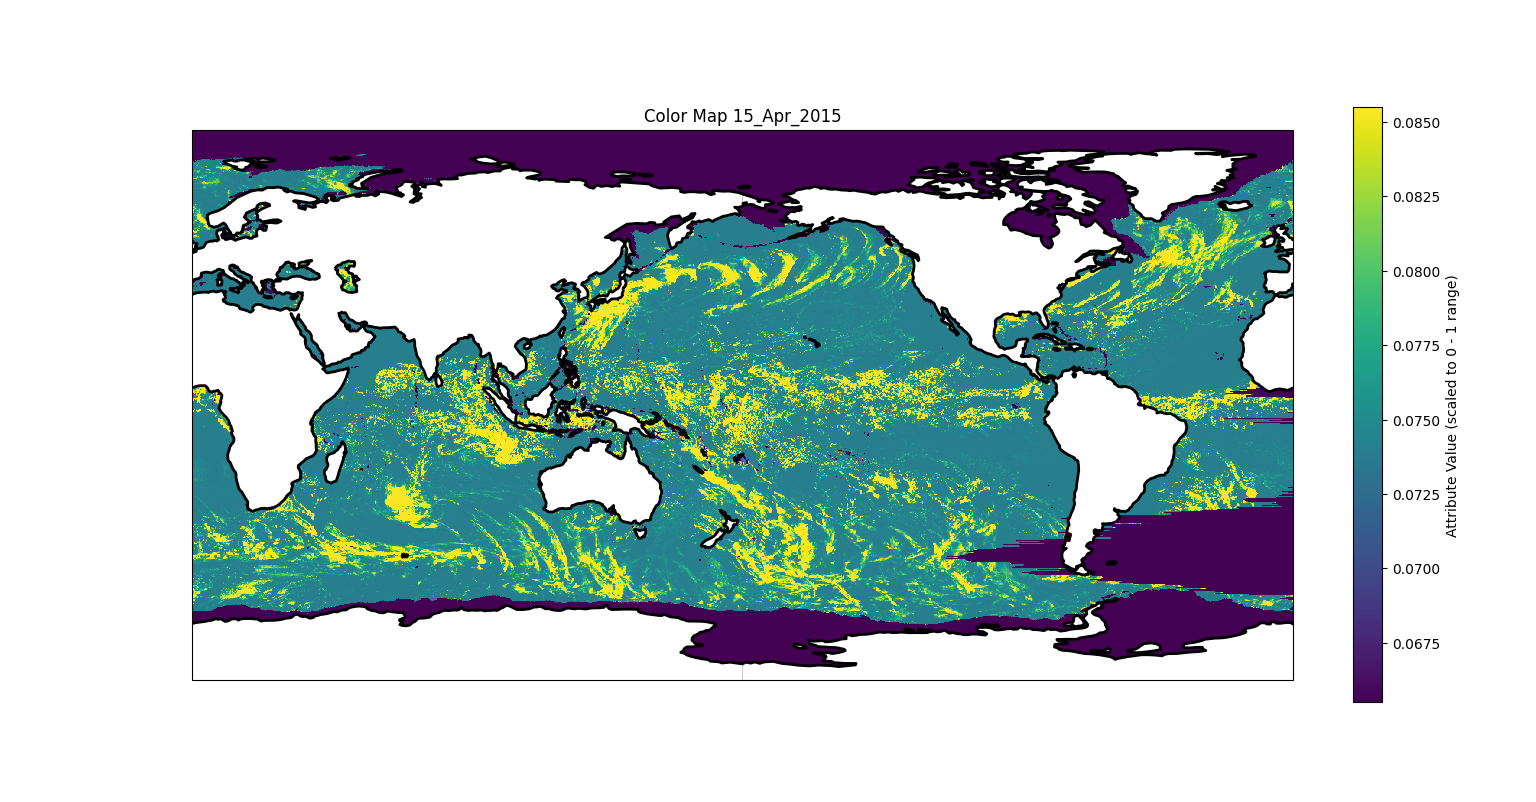
\includegraphics[width=1\linewidth]{Figure_0.png}
        \caption{April 15}
        \label{fig:enter-label}
    \end{figure}
    
    
    \begin{figure}
        \centering
        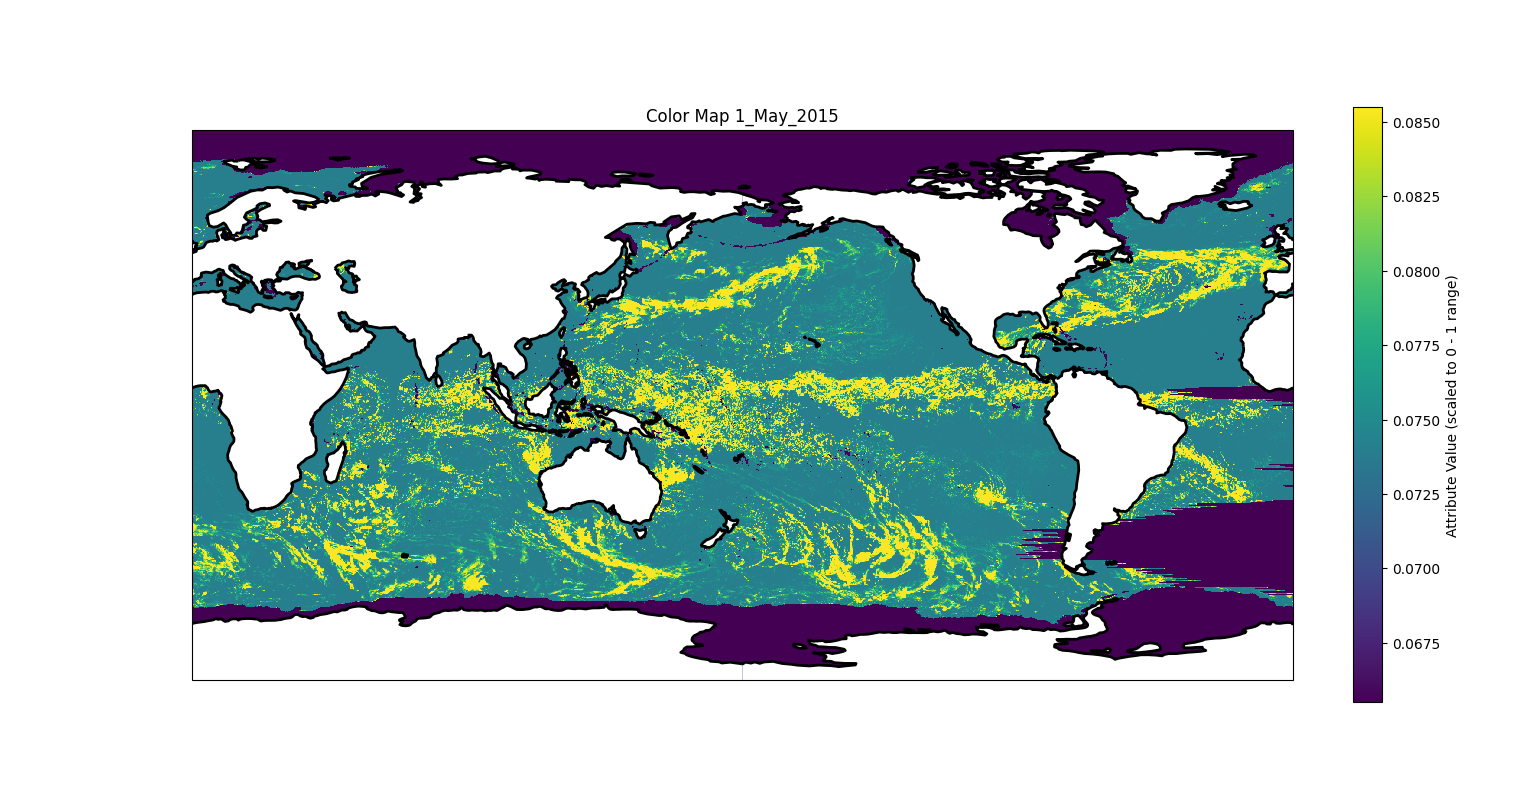
\includegraphics[width=1\linewidth]{Figure_1.png}
        \caption{May 1}
        \label{fig:enter-label}
    \end{figure}
    
    
  
     \begin{figure}
         \centering
         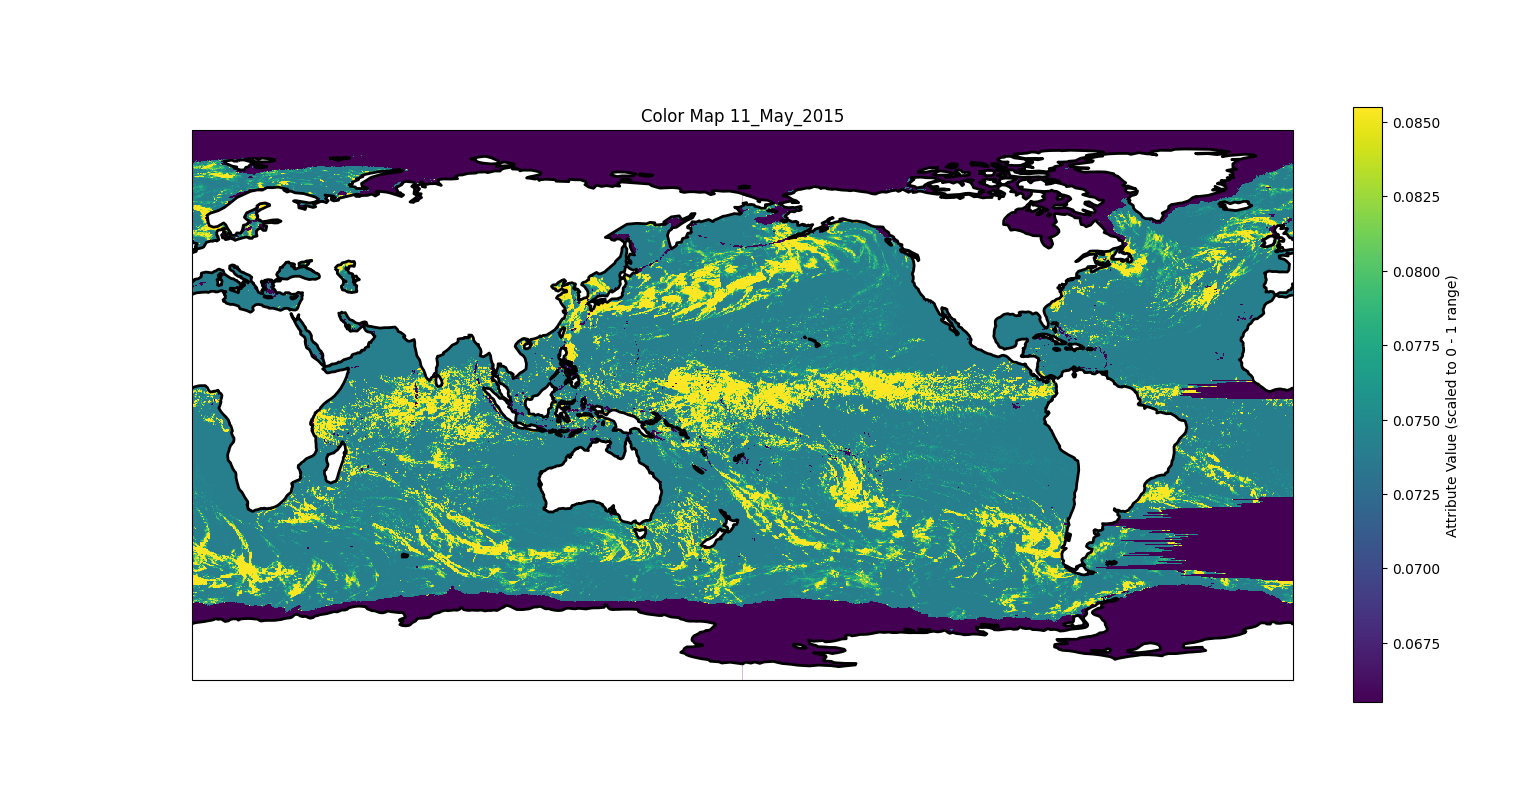
\includegraphics[width=1\linewidth]{Figure_2.png}
         \caption{May 11}
         \label{fig:enter-label}
     \end{figure}
    
    
    
    \begin{figure}
        \centering
        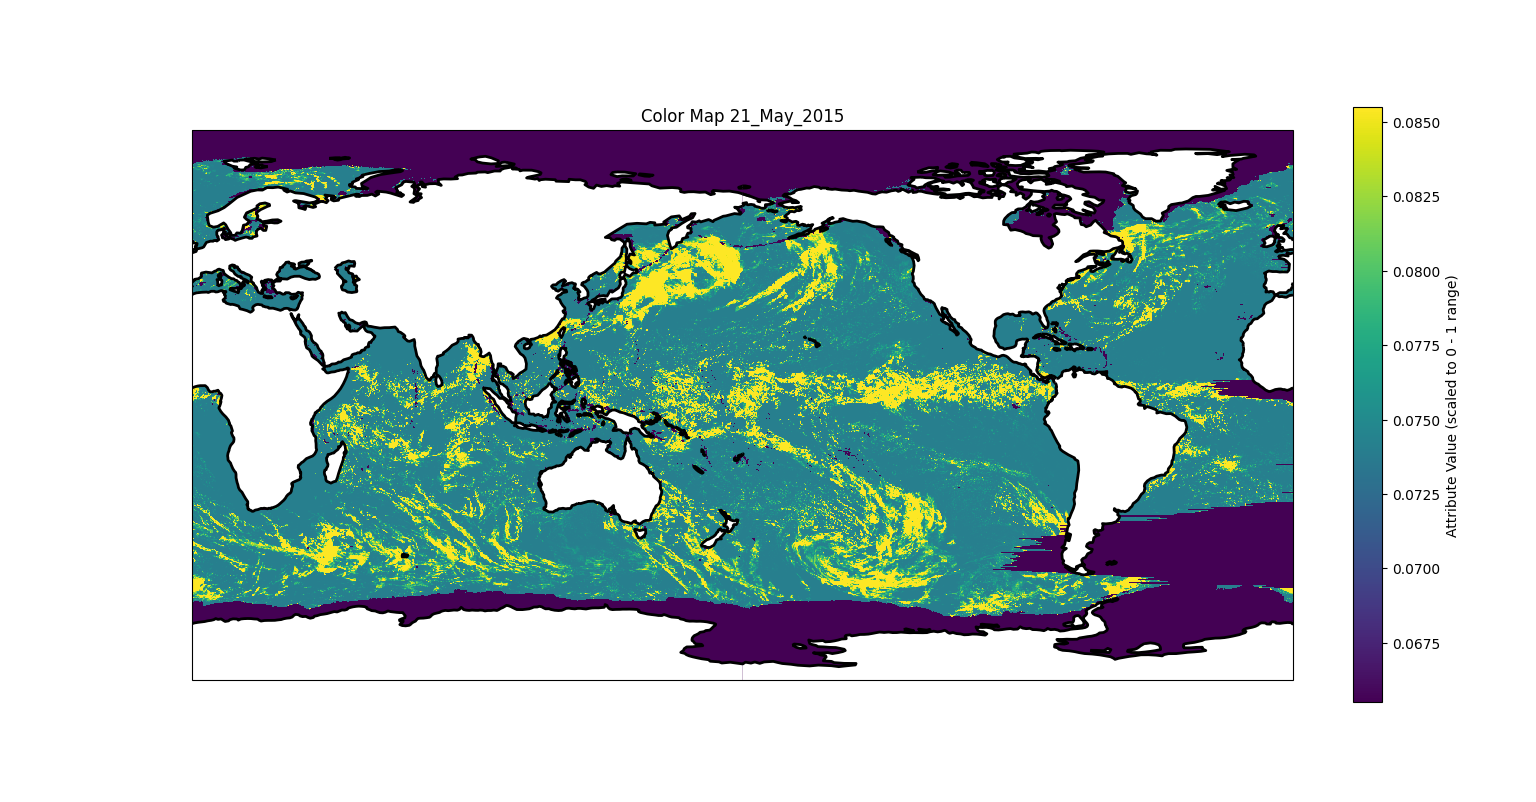
\includegraphics[width=1\linewidth]{Figure_3.png}
        \caption{May 21}
        \label{fig:enter-label}
    \end{figure}
    
    
    \begin{figure}
        \centering
        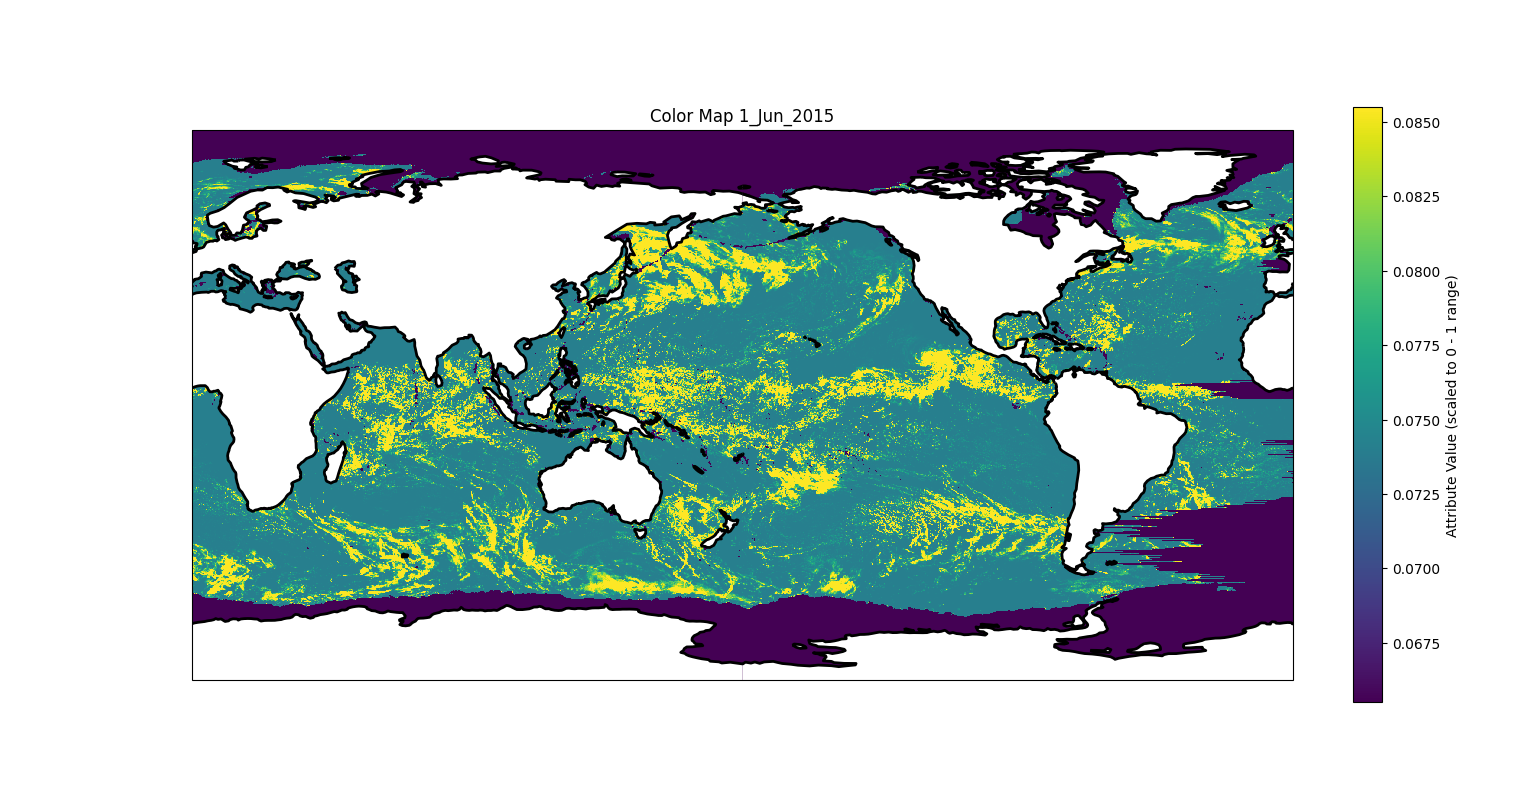
\includegraphics[width=1\linewidth]{Figure_4.png}
        \caption{June 1}
        \label{fig:enter-label}
    \end{figure}

    \begin{figure}
        \centering
        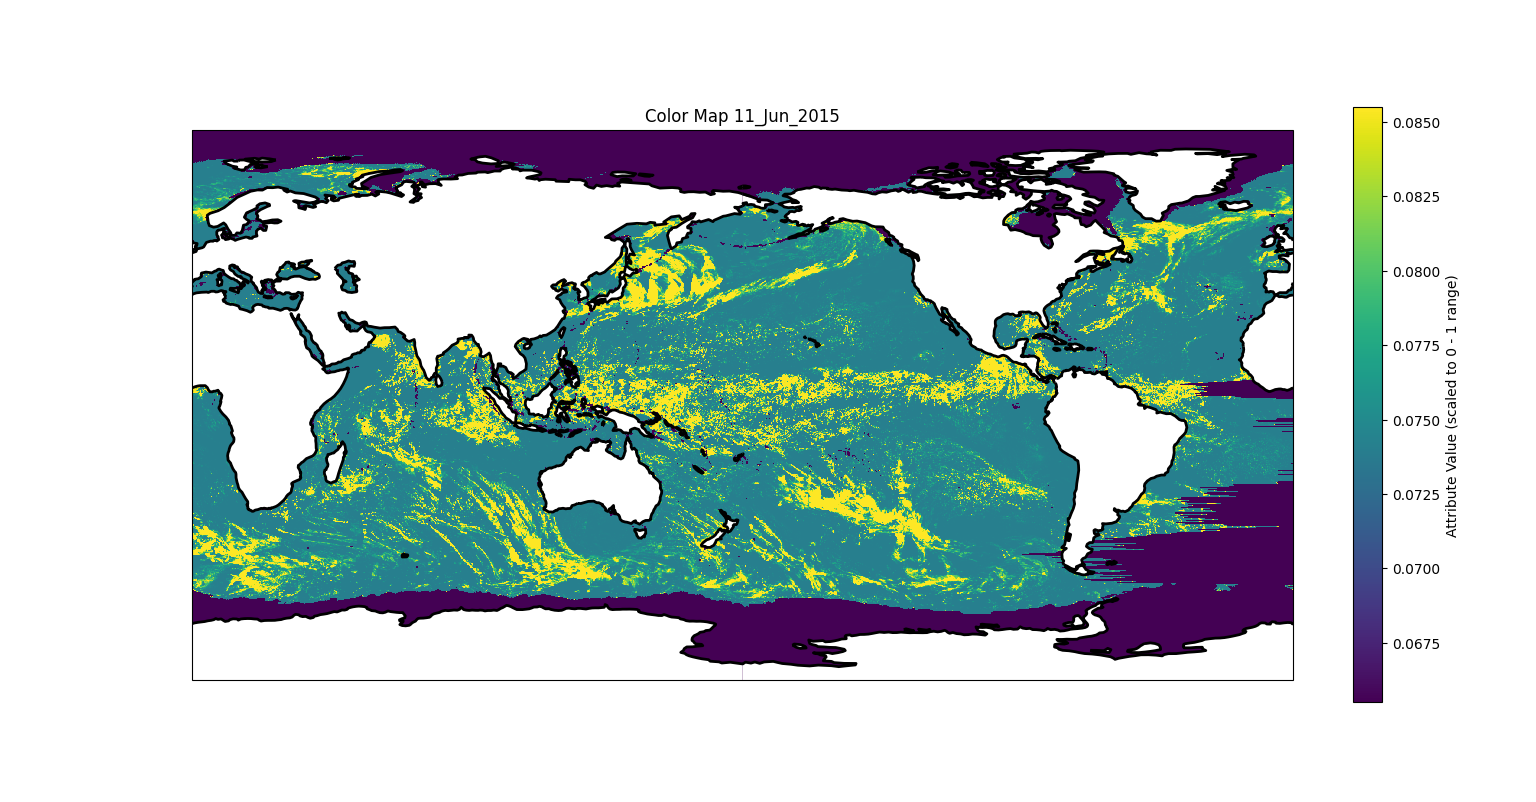
\includegraphics[width=1\linewidth]{Figure_5.png}
        \caption{June 11}
        \label{fig:enter-label}
    \end{figure}

    \begin{figure}
        \centering
        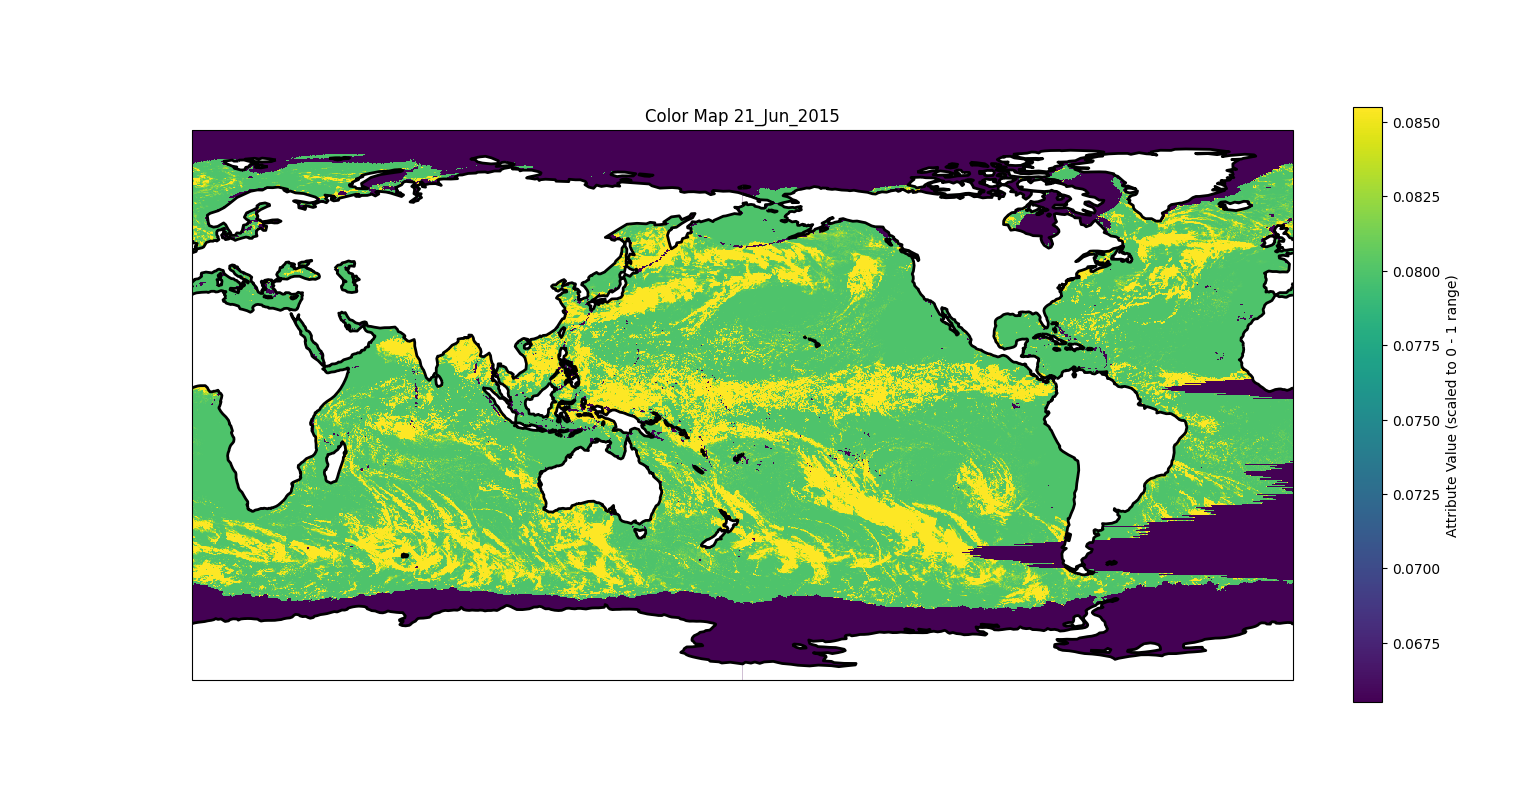
\includegraphics[width=1\linewidth]{Figure_6.png}
        \caption{June 21}
        \label{fig:enter-label}
    \end{figure}




\item \textbf{Python code for creating color map visualizations: \\}

 

\textbf{Cartopy} was used to setup the map and land-mass of continents on the map. Coast-lines were added to the map to clearly separate the land from the ocean data plot.\\

The datasets (.txt files) were processed to remove meta data and the lines ending with **line too long** were also processed to remove the invalid string.\\

Each line of data was read into a 720x1440 array-like variable named ocean data. Wherever the lines were too small, I inserted -999 to indicate absence of value. Later, these -999 were also replaced with -2 to avoid colour scale problems while colouring the map. Otherwise, --999 data points get blue colour and everthing else gets yellow color making the map monotonous at regions and also difficult to read.\\ 

Viridis color scale was used for the color maps. various other color scales were also tried like jet, cividis, ocean. At the end, I decided to stick with viridis as it shows the monsoon patterns well when compared to other color-scales.\\

Matplotlib, specifically the pcolormesh function was used to plot the color maps. The function in code takes a total of 6 arguments namely, longitudes, latitudes, ocean data (2d list array), cmap (the color mapping to be used), and vmin, vmax to specify the scale range. vmin and vmax was adjusted by trial and error, to optimize the output such that the color map shows the trend clearly. I have tried different colormaps like continuous, logarithmic, and discrete color maps. I finally chose to stick with continuous color maps as the plots came out to be better and adjustiing vmin and vmax was easier for continuos than for logarithmic and discrete. The code for all 3 can be found in the same file. Logarithmic and discrete colormap plotting functions have been commented. They can be uncommented and run for testing on your machine. Please comment the continuous colormap plotting function while doing the above.    
\end{enumerate}


\begin{thebibliography}{00}

\bibitem{b1} This website contains ocean dataset in different formats for free download and use. It provides us with many options to choose from, like 3-day-composite, monthly and contains datasets pertaining to different classes like surface rainfall, surface temperature.
https://las.incois.gov.in/ \\

\bibitem{b2} This is the official website maintained by U.S. state government of Maryland State. It contains the crash report data of all the vehicle crashes in Montgomery county of Maryland, from the year 2015 to 2023, which is created by combining multiple crash report databases together.
https://www.nhtsa.gov/sites/nhtsa.gov/files/documents/acrsfieldreference.pdf/ \\

\bibitem{b3} This document describes the crash report dataset of Maryland State. This is different from the original dataset.
https://www.nhtsa.gov/sites/nhtsa.gov/files/documents/acrsfieldreference.pdf/ \\

\bibitem{b4} This is documentation of the library plotly used for constructing a parallel co-ordinate plot 
https://plotly.com/javascript/parallel-coordinates-plot/ \\

\bibitem{b5} This is documentation of the library D3.js used for constructing a parallel co-ordinate plot 
https://d3-graph-gallery.com/graph/treemap_basic.html/ \\

\end{thebibliography}
\end{document}
